% Configuración del documento y paquetes
\documentclass[12pt,a4paper]{article}
\usepackage[english,spanish]{babel}
\usepackage[utf8]{inputenc}
\usepackage[T1]{fontenc}
\usepackage{amsmath}
\usepackage{svg}
\usepackage{graphicx}
\usepackage[colorinlistoftodos]{todonotes}
\usepackage[top=1.5cm, bottom=2.0cm, left=1.50cm, right=1.50cm]{geometry}
\usepackage[nottoc]{tocbibind}
\usepackage{amssymb}
\usepackage{hyperref}
\usepackage{textcomp}
\usepackage{multicol} 
\usepackage{longtable} 
\usepackage[printonlyused,withpage]{acronym}
\usepackage[justification=centering]{caption}
\usepackage{afterpage}
\usepackage{subfig}
\usepackage[export]{adjustbox}
\usepackage{float}

\usepackage{appendix}
\renewcommand{\appendixname}{Anexos}
\renewcommand{\appendixtocname}{Anexos}
\renewcommand{\appendixpagename}{Anexos}

\usepackage{listings}
\usepackage{color}
\definecolor{codegreen}{rgb}{0,0.6,0}
\definecolor{codegray}{rgb}{0.5,0.5,0.5}
\definecolor{codepurple}{rgb}{0.58,0,0.82}
\definecolor{backcolour}{rgb}{0.95,0.95,0.92}
\definecolor{gray75}{gray}{.75}
\lstdefinestyle{mystyle}{
    backgroundcolor=\color{backcolour},   
    commentstyle=\color{codegreen},
    keywordstyle=\color{magenta},
    numberstyle=\tiny\color{codegray},
    stringstyle=\color{codepurple},
    basicstyle=\footnotesize,
    breakatwhitespace=false,         
    breaklines=true,                 
    captionpos=b,                    
    keepspaces=true,                 
    numbers=left,                    
    numbersep=5pt,                  
    showspaces=false,                
    showstringspaces=false,
    showtabs=false,                  
    tabsize=2,
    literate=
  {á}{{\'a}}1 {é}{{\'e}}1 {í}{{\'i}}1 {ó}{{\'o}}1 {ú}{{\'u}}1
  {Á}{{\'A}}1 {É}{{\'E}}1 {Í}{{\'I}}1 {Ó}{{\'O}}1 {Ú}{{\'U}}1
  {à}{{\`a}}1 {è}{{\`e}}1 {ì}{{\`i}}1 {ò}{{\`o}}1 {ù}{{\`u}}1
  {À}{{\`A}}1 {È}{{\'E}}1 {Ì}{{\`I}}1 {Ò}{{\`O}}1 {Ù}{{\`U}}1
  {ä}{{\"a}}1 {ë}{{\"e}}1 {ï}{{\"i}}1 {ö}{{\"o}}1 {ü}{{\"u}}1
  {Ä}{{\"A}}1 {Ë}{{\"E}}1 {Ï}{{\"I}}1 {Ö}{{\"O}}1 {Ü}{{\"U}}1
  {â}{{\^a}}1 {ê}{{\^e}}1 {î}{{\^i}}1 {ô}{{\^o}}1 {û}{{\^u}}1
  {Â}{{\^A}}1 {Ê}{{\^E}}1 {Î}{{\^I}}1 {Ô}{{\^O}}1 {Û}{{\^U}}1
  {œ}{{\oe}}1 {Œ}{{\OE}}1 {æ}{{\ae}}1 {Æ}{{\AE}}1 {ß}{{\ss}}1
  {ű}{{\H{u}}}1 {Ű}{{\H{U}}}1 {ő}{{\H{o}}}1 {Ő}{{\H{O}}}1
  {ç}{{\c c}}1 {Ç}{{\c C}}1 {ø}{{\o}}1 {å}{{\r a}}1 {Å}{{\r A}}1
  {€}{{\euro}}1 {£}{{\pounds}}1 {«}{{\guillemotleft}}1
  {»}{{\guillemotright}}1 {ñ}{{\~n}}1 {Ñ}{{\~N}}1 {¿}{{?`}}1
}
\renewcommand{\lstlistingname}{Listado}
\lstset{style=mystyle}

\definecolor{maroon}{rgb}{0.5,0,0}
\definecolor{darkgreen}{rgb}{0,0.5,0}
\lstdefinelanguage{XML}
{
  %basicstyle=\ttfamily,
  morestring=[s]{"}{"},
  morecomment=[s]{?}{?},
  morecomment=[s]{!--}{--},
  commentstyle=\color{darkgreen},
  moredelim=[s][\color{black}]{>}{<},
  moredelim=[s][\color{red}]{\ }{=},
  stringstyle=\color{blue},
  identifierstyle=\color{maroon}
}

% Configuración de los márgenes del documento
\usepackage{vmargin}
\setpapersize{A4}
\setmargins{2.5cm} % margen izquierdo
{1.5cm}            % margen superior
{16.6cm}           % anchura del texto
{23.42cm}          % altura del texto
{16pt}             % altura de los encabezados
{1cm}              % espacio entre el texto y los encabezados
{0pt}              % altura del pie de página
{2cm}              % espacio entre el texto y el pie de página

% Configuración de cabecera y pie de página
\usepackage{fancyhdr}
\pagestyle{fancy}
\fancyhf{}
\fancyhead[L]{\nouppercase{\leftmark}}
\fancyfoot[C]{Página \thepage}
\renewcommand{\headrulewidth}{0.5pt}
\renewcommand{\footrulewidth}{0.5pt}
\hypersetup{
    colorlinks=true,
    linkcolor=black,
    filecolor=magenta,      
    urlcolor=blue,
    linkbordercolor=white
}
% diccionario de acrónimos
\usepackage[acronym,toc,shortcuts]{glossaries}
\setlength{\glsdescwidth}{0.8\textwidth}
\makeglossaries
\newacronym{GFLOPS}{GFLOPS}{Giga Floating Point Operations Per Second}
\newacronym{TFLOPS}{TFLOPS}{Tera Floating Operations Per Second}
%\newacronym{}{}{}

% Algoritmos en pseudcódigo 
\usepackage[ruled,linesnumbered,spanish,onelanguage]{algorithm2e}
\SetAlFnt{\footnotesize}
% nuevos comandos (macros)
\newcommand{\seccion}[1]{
\textcolor{blue}{
\hrule height 1.5pt
\section{#1}
\hrule height 1.5pt
\vspace{0.5cm}}
}
\newcommand{\subseccion}[1]{
\textcolor{blue}{\subsection{#1}
\hrule
\vspace{0.5cm}}
}
% Configuración de la portada del documento
\newcommand{\doctitle}{Análisis y clasificación de imágenes médicas mediante redes neuronales}
\newcommand{\docauthor}{Gonzalo Caparrós Laiz}
\newcommand{\docdate}{Junio, 2020}
\newcommand{\docdirector}{Dr. D. Gregorio Bernabé García y Dr. D. José Manuel García Carrasco}

\title{\doctitle}
\author{\docauthor}
\date{\docdate}
% Documento 
\begin{document}
\renewcommand*\listtablename{Índice de tablas}
\renewcommand\spanishtablename{Tabla}
\glsunsetall

\newcommand*{\blankpage}{%
\vspace*{\fill}
{\centering Esta página ha sido intencionadamente dejada en blanco\par}
\vspace{\fill}}
% *********************** Portada del Documento
\begin{titlepage}
\begin{center}
\begin{figure}[ht]
\centering
\includegraphics[width=0.5\textwidth]{img/escudo}
\end{figure}
\vspace{1cm}
\begin{Large}
\textbf{Universidad de Murcia\\
Facultad de Informática\\}
\vspace{0.5cm}
GRADO EN INGENIERÍA INFORMÁTICA\\
\vspace{1.0cm}
\textbf{\doctitle}
\end{Large}
\vspace{1.0cm}
\hrule
\vspace{0.2cm}
\begin{large}
\textbf{Trabajo Fin de Grado realizado por:}\\\docauthor\\
\vspace{0.2cm}
\textbf{Bajo la dirección de:}\\
\docdirector\\
\vspace{0.2cm}
\docdate\\
\end{large}
\vspace{0.5cm}
\hrule
\vspace{1cm}
\end{center}
\end{titlepage}
\pagenumbering{roman}
% *********************** Fin Portada del Documento
\renewcommand{\headrulewidth}{0.0pt}
\renewcommand{\footrulewidth}{0.0pt}
\fancyhead[L]{}
\fancyfoot[C]{}
\newpage
\blankpage
%**************************************************
\newpage
\fancyhead[L]{\nouppercase{\leftmark}}
\fancyfoot[C]{Página \thepage}
\renewcommand{\headrulewidth}{0.5pt}
\renewcommand{\footrulewidth}{0.5pt}
\tableofcontents

\newpage
\listoffigures

\newpage
\listoftables

\newpage
\pagenumbering{arabic}
\section*{Declaración firmada sobre originalidad del trabajo}
\fancyhead[L]{Declaración firmada sobre originalidad del trabajo}
\addcontentsline{toc}{section}{Declaración firmada sobre originalidad del trabajo}

D./Dña \docauthor, con DNI 00000000A, estudiante de la titulación de Grado en Ingeniería Informática de la Universidad de Murcia y autor del TF titulado ''\doctitle ´´.
\bigskip
\bigskip

De acuerdo con el Reglamento por el que se regulan los Trabajos Fin de Grado y de Fin de Máster en la Universidad de Murcia (aprobado C. de Gob. 30-04-2015, modificado 22-04-2016 y 28-09-2018), así como la normativa interna para la oferta, asignación, elaboración y defensa de los Trabajos Fin de Grado y Fin de Máster de las titulaciones impartidas en la Facultad de Informática de la Universidad de Murcia (aprobada en Junta de Facultad 27-11-2015)
\bigskip
\bigskip

DECLARO:
\bigskip
\bigskip

Que el Trabajo Fin de Grado presentado para su evaluación es original y de elaboración personal. Todas las fuentes utilizadas han sido debidamente citadas. Así mismo, declara que no incumple ningún contrato de confidencialidad, ni viola ningún derecho de propiedad intelectual e industrial.
\bigskip
\bigskip

Murcia, a 23 de Junio de 2020
\begin{figure}[H]
\centering
\includegraphics[width=0.15\textwidth]{img/firma}
\end{figure}
Fdo.: \docauthor \\
Autor del TF

\newpage
\section*{Resumen}
\fancyhead[L]{Resumen}
\addcontentsline{toc}{section}{Resumen}
En medicina hay trabajos muy tediosos que requieren mucho tiempo de profesionales, como por ejemplo el diagnóstico de enfermedades cardiacas, en el que primero hay que hacer un proceso de señalar las partes de un corazón para luego poder obtener un diagnóstico.
\bigskip

La inteligencia artificial ~\cite{wiki:ai} son algoritmos que intenta simular el comportamiento humano, una forma de intentar hacer eso ha sido la programación tradicional mediante reglas u órdenes, para especificar el comportamiento de un programa en todo momento. Con el paso del tiempo se han planteado situaciones para las que esta forma de enfrentarse a los problemas ya no es factible o directamente imposible debido a la gran cantidad de posibilidades que hay. Un enfoque para solucionar este problema es hacer algoritmos en los que no sea necesario dar las reglas explícitas de cómo resolver un problema, sino que el algoritmo aprenda a resolver el problema. El \textit{machine learning} es un algoritmo que, a partir de unos datos de entrada, aprende a resolver el problema que representan esos datos de entrada, mediante prueba y error.
\bigskip

Hay principalmente tres formas para hacer que un algoritmo aprenda \cite{wiki:ml}. En el aprendizaje supervisado y en el aprendizaje no supervisado hay un conjunto de datos del que se aprende, la diferencia es que en el primero los datos están etiquetados mientras que en el segundo no están etiquetados. En aprendizaje por refuerzo, no hay un conjunto de datos del que entrenar, la entrada consiste en recompensas y penalizaciones que reciben los agentes, en este caso el objetivo es maximizar la recompensa. En el aprendizaje supervisado, el conjunto de entrada se divide en tres subconjuntos de entrenamiento, validación y test, donde el primero se usa para ajustar los valores del modelo y los últimos para la evaluación del modelo.
\bigskip

Un tipo de \textit{machine learning} son las redes neuronales, que consisten neuronas artificiales \cite{wiki:ann} agrupadas en capas, donde la salida de una neurona está conectada con las neuronas de la capa siguiente y la entrada de la neurona es la salida de las neuronas de la capa anterior.
\bigskip

Aunque estos algoritmos ya se conocían hace tiempo no ha sido posible hacer uso de ellos debido a la gran capacidad de cómputo requerido por estos. Con el avance la capacidad de cómputo en los procesadores y la tecnología, ya es posible hacer uso de estos algoritmos en un tiempo razonable.
\bigskip

Sin embargo, aunque haya habido importantes avances en la tecnología para poder implementar modelos que tengan muy buenos resultados, estos modelos son muy grandes y se requieren de máquinas muy potentes y con muchos recursos para poder entrenarlas, estas máquinas suelen tener precios muy elevados. Con el objetivo de poder hacer uso de estas arquitecturas tan potentes sin necesidad de hacer uso de máquinas tan potentes se puede usar \textit{transfer learning} para aprovecharlas. \textit{Transfer learning} \cite{wiki:tl} consiste en partir de un modelo entrenado, eliminar las últimas capas y reentrenarlas para que resuelvan otro problema. \textit{Transfer learning} tiene la ventaja de que requiere menos recursos pero dependiendo del caso se puede obtener mejor o peor precisión que con un modelo específico para ese problema. 
\bigskip

Además de la arquitectura del modelo que se entrena y su ajuste, también es importante tener en cuenta diferentes procedimientos y técnicas que se pueden usar para obtener mejor precisión, como la distorsión de los datos de entrada o técnicas como \textit{random forest} u organizar un conjunto de modelos en cascada. En distorsión de datos se aplican modificaciones a los datos de entrada para mejorar la calidad de estos o si los datos son reducidos para aumentarlos, en el caso de imágenes se pueden aplicar rotaciones o cortes. En \textit{random forest} \cite{wiki:rf} se construye un árbol de decisión que consiste en ir tomando decisiones más simples hasta dar una solución final. La técnica de cascada \cite{wiki:cc} es parecida a \textit{random forest} pero en este caso en cada decisión se dice si la imagen a clasificar es de una clase o no.
\bigskip

El objetivo de este trabajo es buscar una solución para la clasificación de enfermedades cardiacas en el \textit{dataset} \textit{ACDC} \cite{acdcdataset} usando \textit{transfer learning}. Se usa como referencia el \textit{paper} \textit{Automatic Segmentation and Disease Classification Using Cardiac Cine MR Images} ~\cite{DBLP:journals/corr/abs-1708-01141}, en el que proponen una solución para este problema. La forma de realizar el trabajo es realizar distintas pruebas para encontrar la opción más interesante que obtiene el mejor resultado.
\bigskip

En este trabajo se ha utilizado el \textit{framework TensorFlow} para hacer las diferentes pruebas de \textit{transfer learning}. Se ha usado la herramienta incluida en el \textit{framework}, \textit{TensorFlow Hub}, que es un repositorio de modelos entrenados para aplicar \textit{transfer learning}. En esta herramienta todos los modelos han sido entrenados en el \textit{dataset} \textit{ImageNet} \cite{imagenet} con 1000 clases. Para hacer el entrenamiento se ha usado la técnica de \textit{bottleneck} que consiste en hacer un paso previo al entrenamiento, en este paso se obtienen los valores del tensor de salida de todos las imágenes de entrada, a los que se les denomina \textit{bottleneck}. Después estos \textit{bottlenecks} son usados como entrada de un pequeño modelo que es el que realmente se entrena.
\bigskip

Antes de trabajar con el \textit{dataset} principal de este trabajo (\textit{ACDC}) se han hecho algunas pruebas con algunos \textit{datasets} y modelos de prueba para analizar el comportamiento y después aplicarlo al \textit{dataset} principal. La primera prueba consiste en hacer un entrenamiento completo con la arquitectura \textit{AlexNet} en el \textit{dataset} \textit{cifar 10} (10 clases), que resulta en una precisión del 68\%.
\bigskip

A continuación se usa \textit{transfer learning}, en estas pruebas se elimina la última capa del modelo de partida y se añaden: una nueva capa totalmente conectado, una capa \textit{softmax} y se reentrenan esas capas. El modelo preentrenado es \textit{inception v3} y los \textit{datasets} usados son \textit{cifar 10} (3 clases), \textit{flowers} (5 clases), \textit{cifar 10} (10 clases), \textit{cifar 100} (20 clases) y \textit{cifar 100} (100 clases) que producen unos resultados de 94\%, 91\%, 79\%, 64\% y 52\% de precisión respectivamente. Con estas pruebas y la previa se pueden ver dos características principalmente.
\bigskip

Comparando el resultado de hacer un entrenamiento completo con la prueba similar usando el mismo \textit{dataset}, el primero obtiene una mejor precisión porque se está entrenando un modelo completo (86\% de precisión comparado con 79\% de precisión obtenido usando \textit{transfer learning}). También viendo los resultados usando \textit{transfer learning} se pueden observar que cuantas más clases se intentan clasificar, peor es el resultado.
\bigskip

En las siguientes pruebas se ejecutan las mismas pruebas anteriores pero en vez de usar \textit{inception v3} \cite{DBLP:journals/corr/SzegedyVISW15} como el modelo base se usa \textit{resnet v2 512}. En estas pruebas se obtienen unos resultados muy similares a las pruebas anteriores, alrededor del 3\% de mejora.
\bigskip

La prueba a continuación consiste en añadir 3 capas totalmente conectadas en vez de añadir una solo. En este caso se obtienen resultados similares a los anteriores pero necesitando más iteraciones para alcanzarlos.
\bigskip

A continuación se prueba eliminado más de una capa al final de modelo, primero se prueba eliminando 2 capas y después 3 capas. En el caso de eliminar 2 capas se obtienen resultados similares a las pruebas previas. En el caso de eliminar 3 capas se puede apreciar un empeoramiento de la precisión, por lo tanto no es una buena idea eliminar más de 2 capas para hacer \textit{transfer learning} en el modelo \textit{inception v3}.
\bigskip

Después de hacer pruebas con \textit{datasets} de ejemplo se empieza a usar el \textit{dataset} principal. El \textit{dataset} \textit{ACDC} consiste en 100 imágenes de resonancias magnéticas (\textit{MRI}). Cada \textit{MRI} es una serie de fotogramas tridimensionales del corazón del paciente. Cada paciente es etiquetado en una enfermedad (\textit{myocardial infarction}, \textit{dilated cardiomyopathy}, \textit{hypertrophic cardiomyopathy}, \textit{abnormal right ventricle}) o normal.
\bigskip

La primera prueba con este \textit{dataset} consiste en extraer todos los fotogramas y dividir estos fotogramas tridimensionales en imágenes bidimensionales. Con todas esas imágenes hacer los conjuntos de entrenamiento, validación y test. Para el modelo de partido se usa \textit{inception v3} al que se le elimina una capa al final y se le añade una nueva capa totalmente conectada que será entrenada. El resultado de esta prueba es 99\% de precisión, pero hay un problema en esta prueba, al haber hecho la división de los conjuntos de entrenamiento, validación y test sin tener en cuenta que hay imágenes relacionadas por pacientes, ha surgido \textit{overfitting}.
\bigskip

Para solucionar el problema del \textit{overfitting} se hace básicamente la misma prueba pero en este caso la división de los conjuntos se hace de forma correcta. Es decir, teniendo en cuenta que la división debe de ser por paciente. Por lo tanto todas las imágenes de un mismo paciente deben de estar en el mismo conjunto. Y no puede haber imágenes de un mismo paciente en conjuntos distintos. El resultado haciendo esto es de 63\% de precisión, que no es lo suficientemente bueno.
\bigskip

En la siguiente prueba en vez de coger todas las imágenes de todos los pacientes se coge únicamente una imagen por paciente. De esta manera la precisión obtenida es del 43\%.
\bigskip

Después de estas pruebas se empiezan a usar diferentes enfoques para intentar mejorar la precisión. Para esta prueba el primero paso es hacer un modelo que agrupe las clases en subsets y aprenda a diferenciar esos subsets. Esta idea es la base para implementar la siguiente prueba. La prueba consiste en organizar una serie de modelos en cascada. Esto es, el primer modelo diferencia entre una clase y el resto, el siguiente entre las que quedan y otra. Se sigue así hasta que un modelo identifique la clase como la que hace referencia o solo queden dos clases. El resultado de esta prueba es 63\% de precisión, que es muy parecido al mejor resultado que ya se había obtenido, por lo que este enfoque no ha supuesto ningún avance.
\bigskip

A continuación se hace una pruebo incluyendo una mejora que consiste en, partir de los resultados de un modelo para todas las imágenes de un mismo paciente, ponerlas todas en común y quedarse con la clase que más se repita. Esto se aplica a dos pruebas. En el caso de añadir una capa obtengo una mejora del 8\% en la precisión (71\%). En el caso de la prueba de cascada se obtienen peores resultados (57\%).
\bigskip

Por último se aplica distorsión a todas las imágenes de entrada y ejecuto todas las pruebas previas. La distorsión consiste en rotar las imágenes 90, 180 y 270 grados cada una. Con esto se obtiene una pequeña mejora en general, excepto en las pruebas que dan como resultado la clase más repetida para todas las imágenes de un mismo paciente, en las que se obtiene una mejora significativa. En esas pruebas obtengo un 86\% de precisión.
\bigskip

Finalmente después de trabajar en las diferentes pruebas los mejores resultados obtenidos son los últimos. En concreto las pruebas de añadir una capa y cascada, usando el modelo \textit{inception v3} como modelo base, usando distorsión y teniendo en cuenta la clase más repetida para todas las imágenes de un mismo paciente. Entre estos dos resultados se escoge el de la prueba de añadir una capa ya que es más simple y por lo tanto tiene la ventaja de que requiere menos recursos.
\bigskip

En conclusión en el campo de \textit{machine learning} hay muchos factores que pueden tener un efecto en el resultado final, como la arquitectura del modelo, el \textit{dataset} de entrada, los parámetros del modelo o los diferentes enfoques con los que se pueden solucionar los problemas. En este trabajo se ha comprobado que todos estos factores son importantes. Después de enfocar el problema desde diferentes enfoques el mejor resultado que se ha obtenido ha sido 86\% de precisión.
\bigskip

Como trabajo futuro para mejorar los resultados se proponen dos vías: usar un modelo de partida que procese los datos de entrada como imágenes tridimensionales y usar un enfoque en el que problema se divida en dos subtareas, primero segmentar las imágenes del corazón y a continuación hacer una predicción de la enfermedad.

\newpage
\section*{Extended Abstract}
\fancyhead[L]{Extended Abstract}
\addcontentsline{toc}{section}{Extended Abstract}
Certain tasks in medicine may be tedious and require a lot of time from professionals, like the diagnosis of cardiac diseases, in which the process requires first to segmentate the heart parts and then make a diagnosis.
\bigskip

Artificial intelligence are algorithms \cite{wiki:ai} that try to simulate human behavior. Rule based programs have traditionally been used to do so, determining the behavior of a program at any time. Over time tasks have arisen for which rule based programs are no longer feasible or directly impossible due to the huge amount of possibilities that the program has to deal with. An approach to solve this problem is to make an algorithm in which instructions are not explicitly given to solve the problem, but rather the algorithm learns by itself to solve the problem, this is called machine learning. Machine learning \cite{wiki:ml} algorithms take input data that represent a problem to solve, and use them to learn the to solve the problem through trial and error.
\bigskip

There are mainly three types of learning algorithms \cite{wiki:ml} . In supervised learning and unsupervised learning an input dataset is provided for learning, the difference lies in the labelling, in the first type the data is labeled while in the last is not. In reinforcement learning there is not an input dataset, the input consists in rewards and penalties agents receive while exploring an environment. The agents receive rewards if they approach the goal or a penalty otherwise. The input dataset is split in three subsets: training, validation and test. The training set is used to fit the values of the model and the last two to evaluate the model.
\bigskip

Neural networks \cite{wiki:ann} are one type of machine learning, which consist in artificial neurons arranged in layers, where the output of one neuron is connected to the input of the neurons of the next layer and the input of one neuron is the output of the neurons of the previous layer.
\bigskip

Although these algorithms were already known a long time ago they could not be used due to the large amount of compute power needed to run this type of algorithms. With the increase of the compute power of processors and technology, nowadays it is possible to run these algorithms in a reasonable time.
\bigskip

Even though there has been important development in the technology to make it possible to run models with very good results, the models are very large and require powerful machines with a lot of resources to be able to train the models, these machines usually cost a lot. With the objective of being able to use these powerful model architectures without the need of very powerful machines transfer learning can be used. Transfer learning consists in using a pretrained model from which the last layers of the neural network are removed and then new layers are retrained to solve a similar problem. Transfer learning has the advantage of not needing very powerful machines to train but depending on the case the model can achieve better or worse than with a model specifically trained to solve the same problem.
\bigskip

In addition to the model architecture and the training, some techniques that can be applied are also important to achieve success solving a task or improving accuracy, such as input data distortion or technique like random forest and arranging models in cascade. In data distortion transformations are applied to the input dataset to improve the quality of them or to make a reduced input dataset larger in this case is called data augmentation. For images some transformations that can be applied are rotation, crop and translation. In a random forest \cite{wiki:rf} a decision tree is built that consists in dividing the problem in steps in which each step the model has to take one simpler decision to eventually give a final solution. Arranging models in cascade \cite{wiki:cc} is similar to random forest but in this casein each decision each model tells if the input belongs to a class or not.
\bigskip

The aim of this Bachelor Thesis is to find a solution for the classification of the cardiac diseases as described in the Automated Cardiac Diagnosis Challenge (ACDC), which also provides a dataset to train a model or use transfer learning. The procedure to achieve this is doing different tests to find the best option that yields the best results.
\bigskip

In this Bachelor Thesis TensorFlow has been used to make the different transfer learning tests. The tool TensorFlow Hub, included in the framework, has been used to perform the transfer learning tests. TensorFlow Hub is a repository of machine learning models trained and prepared to be used with transfer learning in a simple way. All models in the repository have been trained with the ImageNet \cite{imagenet} dataset with 1000 classes. The bottleneck method has been used in the training process. Bottleneck consists in making a previous step in the training process, in which all output values of the input data is calculated for the initial model, these values are called bottlenecks. After this step bottlenecks are used as input for a small model which is what is actually trained.
\bigskip

Before working with the main dataset of this Bachelor Thesis (ACDC) \cite{acdcdataset} I have run some tests on sample data and models to see the behaviour, on simpler environments to then apply them on the main dataset. The first test is a full training of the model architecture AlexNet on the dataset cifar 10 (10 classes), which results in 86\% of accuracy.
\bigskip

Then I start using transfer learning, in the following tests I remove the last layer, add a new fully connected layer, a softmax layer and retrain those layers. I run tests using a pretrained model of inception v3 on the datasets cifar 10 (3 classes), flowers (5 classes), cifar 10 (10 classes), cifar 100 (20 classes) and cifar 100 (100 classes) resulting in 94\%, 91\%, 79\%, 64\% and 52\% of accuracy respectively. With these and the previous tests I can observe two main things.
\bigskip

Comparing the result of the first test with the similar test using the same dataset, the first obtains a better result because of training a full model (79\% accuracy using transfer learning versus 86\% accuracy training a full model). Also comparing the results of the test using transfer learning I can observe the more classes you add the worse the result is.
\bigskip

In the next tests I run the same tests as before but using resnet v2 152 instead of inception v3, obtaining very similar results only getting 3\% better accuracy in each test.
\bigskip

The following test consists in instead of adding just one fully connected layer adding 3 fully connected layers. In this case I obtain similar results to the previous test but needing additional training iterations to reach the same accuracy.
\bigskip

The next tests consist in removing more than one layer from the end of the model. First I try removing 2 layers and then removing 3 layers. In the test removing 2 layers, I obtain similar results to the previous test. In the test removing 3 layers, I can appreciate a reduction in accuracy therefore it is not a good idea to remove more than 2 layers to make transfer learning in the model inception v3.
\bigskip

After running some tests with sample datasets I start using the main dataset. The dataset consists of 100 MRI from 100 patients, each MRI is a series of three-dimensional frames of the heart of the patient. Each patient is labeled with a disease (myocardial infarction, dilated cardiomyopathy, hypertrophic cardiomyopathy, abnormal right ventricle) or normal.
\bigskip

The first test consists in extracting all the frames and split all the 3d images into slides to get a lot of 2d images. Using all that set of 2d images I make 3 sets: train, validation and test. And for the model I use a pretrained inception v3 model which I remove the last layer and add a new one fully connected layer to train. The result of this test is 99\% of accuracy, but in this test there is a problem. This test is not useful as it has a lot of overfitting because the input dataset has not been properly slit.
\bigskip

The next test is basically the same model as before but making the dataset split right. In this case the images are split by patient. Including all the images from the same patient in the same set (train, validation or test) that way images from the same patient can not be in more than one set. With this I can solve the problem of overfitting. The result of this test is 63\% which is not good enough.
\bigskip

The following test consists in instead of using all slices from all patients, using only one slice from each patient. With this I try to reduce the overfitting reducing the number of related samples in the input dataset. This test gets 43\% of accuracy which is not very good, the problem with this test might be that there are not enough samples in the input dataset.
\bigskip

After those tests I start to test different things to try to improve the accuracy. For the next test the first step is to make a model that groups the labels in subsets and learn to identify those sets. This idea is the base to implement the next test. The test consists in arranging a series of models in cascade, which is a decision tree in which in each step the model decides if the input belongs to a class or to the rest and so on till there are only two classes left. The result of this test is 63\% accuracy, this test does not get any progress as the result is very similar to the previous best I had.
\bigskip

The next test consists in training a model but this time I take all the images from the same patient and after running the inference in all of them I get the class that is the most repeated. I do this in combination with two previous tests: the add one layer test and the cascade test. In the case of the add one layer test I get an improvement in accuracy of 8\% (result 71\%), which is a significant improvement. But in the case of the cascade test I get worse results (57\%).
\bigskip

Lastly I apply distortion to all images and run all the previous tests. The distortion consists in rotating all the images 90, 180 and 270 degrees. Doing this I generally get a little improvement in the tests except the tests that take in account the most repeated class in each prediction all the slices of the same patient in which I get an interesting improvement. In those tests I get an accuracy of 86\%.
\bigskip

Finally after working on the tests the best results I got is the latest. Specifically the add one layer and cascade, using inception v3 as the base model, combined with distortion and taking in account the most repeated class per patient. Between these two tests I choose as the best result the add one layer test, because it is simpler and hence it requires less resources to be run.
\bigskip

In conclusion in the field of machine learning there are a lot of factors that can have an effect in the final result such as the architecture of the neural network, the input dataset, the parameters of the model or the different approaches that can be used to solve certain problems. In this Bachelor Thesis I have realized that all those factors are important to obtain a good result. After approaching the problem in different ways the best result I got was 86\%, with the add one layer, using inception v3 as the base model, combined with distortion and taking in account the most repeated class per patient.
\bigskip

As future work I propose two options to improve the accuracy: Using a model that processes the input as 3d images instead as separates images for one dimension. And approaching the problem splitting the problem in two subtasks, first segmetate the heart image and then predict the disease.

\newpage
\section{Introducción}
\fancyhead[L]{\nouppercase{\rightmark}}

Ciertos procedimientos en medicina requieren la dedicación de muchas horas de trabajo de los profesionales del sector, por lo tanto consumen muchos recursos ya sea de tiempo, muy valioso para dar diagnósticos de forma rápida y eficaz, como económicos. Uno de estos procedimientos es el diagnóstico de ciertas enfermedades, los cuales requieren la segmentación de imágenes médicas de distintos órganos y tejidos. En concreto en este trabajo vamos a tratar de la clasificación de las Imágenes por Resonancia Magnética (\textit{MRI}) del corazón y por lo tanto su diagnóstico.
\bigskip

Estas tareas son muy repetitivas siendo esto una ventaja para los programas de inteligencia artificial ya que lo hacen siempre de la misma manera y de forma mucho más rápida que las personas. Este trabajo se basa en el paper \textit{Automatic Segmentation and Disease Classification Using Cardiac Cine MR Images} ~\cite{DBLP:journals/corr/abs-1708-01141} en el que se desarrolla una red neuronal basada en convoluciones dilatadas. En este trabajo se propone una solución al mismo problema pero con un enfoque distinto, partir de una red neuronal ya entrenada en un conjunto de datos distintos y utilizar técnicas de \textit{transfer learning} para resolver el mismo problema que en el paper ~\cite{DBLP:journals/corr/abs-1708-01141}. Se hacen diferentes pruebas y se estudia cual es la mejor solución. En otras palabras se intenta reducir el tiempo de una tarea que hecha por los procedimientos tradicionales sería muy lenta, de esta forma podemos dar un diagnóstico más rápido y a más pacientes. Para llevar a cabo el trabajo se usa el \textit{framework} \textit{TensorFlow} y se utilizan los modelos de partida que se proporcionan en \textit{TensorFlow Hub}, principalmente \textit{resnet} e \textit{inception v3} \cite{DBLP:journals/corr/SzegedyVISW15}.
\bigskip

En los últimos años los avances en inteligencia artificial han tenido un gran impulso que ha hecho que surjan multitud de aplicaciones de esta tecnología, incluyendo casos de uso en medicina. Un factor que ha contribuido al gran avance que ha habido en estas tecnologías son el aumento de la capacidad de cómputo del \textit{hardware}, que ha permitido entrenar grandes modelos, que funcionan muy bien. También otro factor importante es el uso de redes neuronales convolucionales \cite{DBLP:journals/corr/SzegedyVISW15}, que consiguen reducir de forma importante la cantidad de cómputo necesaria para obtener buenos resultados, al contrario que usar capas totalmente conectadas que requieren mucho computo.
\bigskip

Aún así, aumentando la capacidad del \textit{hardware} y reduciendo la necesidad de computo de los modelos, estos siguen necesitando de máquinas muy potentes. Recientemente la técnica de \textit{transfer learning} \cite{wiki:tl} está siendo usada para poder obtener muy buenos resultados sin la necesidad de tener máquinas muy potentes y por lo tanto haciendo posible el uso de la inteligencia artificial en muchos más campos. Esta técnica funciona usando un modelo de partida muy potente que ya ha sido entrenado para resolver un problema al que se le elimina la última capa y se reentrena, esta última capa, para que resuelva un problema parecido. En este trabajo se ha usado esta técnica para cumplir los objetivos.

\newpage
\section{Estado del arte}

\subsection{Inteligencia artificial}
Se entiende por inteligencia artificial \cite{wiki:ai} como los programas que intentan simular el comportamiento humano para resolver un problema. Hay muchos formas de enfocar un programa de inteligencia artificial unas más fáciles de entender como la simbólica, que es un programa basado en reglas que intenta imitar el comportamiento humano, o un enfoque sin símbolos en el que se encontraría el \textit{machine learning}, en el que podemos tener millones de parámetros que entrenar y no saber qué representa cada uno.

\subsection{Machine learning}
Es un tipo de inteligencia artificial sin símbolos que consiste en algoritmos \cite{wiki:ml} que resuelven un problema sin darle instrucciones explícitas de cómo se resuelve el problema. Estos algoritmos construyen un modelo matemático que suele tener millones de parámetros, que se entrenan, difíciles de analizar para saber qué es lo que hace que dé el resultado que da. Generalmente el \textit{machine learning} se usa para resolver problemas para los que no es factible o es muy difícil hacer un algoritmo tradicional.
\bigskip

Para ello parte de unos datos de muestra o datos de entrada de los que aprenderá a resolver el problema que tiene que resolver, mediante repetición de cálculo del error y ajuste del modelo. Estos datos se suelen dividir en tres conjuntos o sets:

\begin{itemize}
\item \textbf{\textit{Training} set}: este set se usa para que el modelo se entrene. Con este set se calculan los errores en el momento del entrenamiento y se usan para ajustar los parámetros del modelo que se está entrenando.
\item \textbf{\textit{Validation} set}: este set se usa durante el entrenamiento para evaluar el modelo y poder ver el progreso.
\item \textbf{\textit{Test} set}: este set se usa al final, cuando el modelo ya ha sido entrenado, para evaluar el modelo con unos datos que nunca hayan sido vistos de ninguna manera por el modelo.
\end{itemize}

Hay principalmente tres formas de hacer que un modelo aprenda \cite{wiki:ml} a resolver el problema cada enfoque es más apropiado para resolver un tipo de problema.

\subsubsection{Aprendizaje supervisado}
El aprendizaje supervisado consiste en aplicar \textit{machine learning} a unos datos de entrada que están etiquetados y por lo tanto el modelo aprenderá a etiquetar esas clases. Aplicaciones comunes del aprendizaje supervisado son la clasificación y regresión. En la clasificación la salida de los modelo es un número limitado de valores que son los que los datos de entrada están etiquetados. En la regresión la salida puede tener cualquier valor numérico en un rango.

\subsubsection{Aprendizaje no supervisado}
El aprendizaje no supervisado consiste en aplicar \textit{machine learning} a unos datos de entrada que no estén etiquetados y el modelo aprenda a encontrar patrones en esos datos y a agruparlos de forma automática.

\subsubsection{Aprendizaje por refuerzo}
El aprendizaje por refuerzo consisten en agentes que se mueven por un entorno realizando acciones obteniendo una recompensa cuando se van acercando a la solución. El objetivo básico es maximizar la recompensa. En este enfoque no es necesario unos datos de entrada etiquetados.

\subsection{Redes Neuronales}
Inspiradas en el funcionamiento de las redes neuronales biológicas \cite{wiki:ann}, una red neuronal es una forma de organizar los modelos de inteligencia artificial para abordar ciertos problemas que son difíciles de resolver con la programación ordinaria basada en ``Reglas'' obteniendo muy buenos resultados en una amplia variedad de tareas como por ejemplo: la visión por ordenador o el reconocimiento de la voz.
\bigskip

Este tipo de inteligencia artificial se organiza en varias capas interconectadas entre sí. Las capas se suelen nombrar como capa de entrada, que es la primera capa, a la que se le pasan directamente los datos de entrada, capa de salida, que es la última capa, la que da el resultado de la predicción que hace la red neuronal y capas ocultas, que son las que están entre la primera y la última.
\bigskip

Las capas de una red neuronal están compuestas por neuronas artificiales.

\begin{figure}[H]
\centering
\includegraphics[width=0.3\textwidth]{img/nn}
\caption{Ejemplo de red neuronal con capa de entrada, capa de salida y una capa oculta.}
\end{figure}

\subsubsection{Neuronas artificiales}
Las neuronas artificiales \cite{wiki:an} son la unidad básica de una red neuronal reciben una entrada y producen una salida. La entrada la reciben de la capa inmediatamente anterior a la capa a la que pertenecen y la salida es la entrada de la capa inmediatamente a continuación. El funcionamiento básico de una neurona es el siguiente: las entradas se multiplican por un peso y se suman, el valor se le aplica una función que dará la salida de la neurona, también llamada función de activación.

%TODO use minipage
\begin{figure}[H]
\centering
\subfloat{{\large $y_{i} = f\left(\sum_{j=0}^{k}w_{ij}x_{j}\right)$}}%
\qquad
\subfloat{{\includegraphics[valign=c, width=0.3\textwidth]{img/neurona} }}%
\caption{Formula de suma de pesos e imagen de una neurona.}
\end{figure}

%TODO son los pesos que
Donde $f$ es la función de activación, $w_{ij}$ son los pesos, $x_{i}$ son las entradas e $y$ es la salida.
\bigskip

%TODO que es x w 
Algunas de las funciones de activación más usadas son las siguientes. En los siguientes apartados $z$ se refiere a la entrada de la función según la fórmula:
\begin{equation*}
z = \sum_{j=0}^{k} w_{j} x_{j}
\end{equation*}

\begin{itemize}
\item \textbf{Función escalonada}: La salida de esta función es 1 si el valor de entrada es mayor que cierto umbral o 0 si está por debajo del umbral.

\begin{figure}[H]
\centering\begin{minipage}[H]{0.5\textwidth}
\large
\begin{equation*}
y = \begin{cases}
1 & si \: z \geq \alpha \\
0 & si \: z < \alpha
\end{cases}
\end{equation*}
\end{minipage}%
\begin{minipage}[t]{0.5\textwidth}
\includegraphics[valign=c, width=0.8\textwidth]{img/escalonada}
\end{minipage}
\caption{Formula y gráfica.}
\end{figure}
%TODO que es alpha y en este caso alpha es 0

\item \textbf{Combinación lineal}: En esta función la salida simplemente se le suma un \textit{bias}. Esta función aplica una transformación lineal a la entrada
%TODO formula

\item \textbf{Sigmoide}: Una función sigmoide es una función matemática que tiene la característica que su curva tiene forma de \textit{s}. Con esta función las entradas negativas tienden a cero y conforme la entrada se acerca a cero la salida va aumentando hasta que el valor de entrada es positivo, conforme se aleja de cero tiende a uno. La función más utilizada es la función logística pero otras funciones matemáticas con forma de \textit{s} también se usan como la tangente o la tangente hiperbólica.

\begin{figure}[H]
\centering\begin{minipage}[H]{0.5\textwidth}
\large
\begin{equation*}
y = \frac{1}{1+e^{-x}}
\end{equation*}
\end{minipage}%
\begin{minipage}[t]{0.5\textwidth}
\includegraphics[valign=c, width=0.8\textwidth]{img/sig}
\end{minipage}
\caption{Formula y gráfica.}
\end{figure}
%TODO en este caso se plot la logistica; usar e bien en el plot

\item \textbf{Rectificador}: Esta función se define como la parte positiva de la entrada. Es decir si la entrada es positiva esa es la salida sin embargo si la entrada es negativa la salida es cero.

\begin{figure}[H]
\centering\begin{minipage}[H]{0.5\textwidth}
\large
\begin{equation*}
y = max(0, x)
\end{equation*}
\end{minipage}%
\begin{minipage}[t]{0.5\textwidth}
\includegraphics[valign=c, width=0.8\textwidth]{img/rectificador}
\end{minipage}
\caption{Formula y gráfica.}
\end{figure}

\end{itemize}

\subsubsection{Tipos de capas}
%TODO extender
Hay distintos tipos de capas con diferentes características y funciones.

\begin{itemize}
\item \textbf{Convolución}: Esta capa es de las más usadas y da nombre al tipo de red que se crea. Funciona seleccionando un conjunto de la entrada y combinando los valores en uno solo mediante una función matemática. De esta forma dichos valores se reducen pero el resultado de salida tiene más información comprimida o más significativa. Es como una simplificación.

\begin{figure}[H]
\centering
\includegraphics[width=0.3\textwidth]{img/c}
\caption{Convolución.}
\end{figure}

\item \textbf{Convolución dilatada}: Es una convolución en la que los valores de entrada no se abordan todos juntos sino que se agrupan en círculos, separados por unos espacios, de esta forma los datos de entrada, a cada una de las neuronas de este tipo de capa, abarcan más.

\begin{figure}[H]
\centering
\includegraphics[width=0.3\textwidth]{img/ac}
\caption{Convolución dilatada.}
\end{figure}

\item \textbf{\textit{Pooling}}: Consiste en agrupar los datos en una dimensión usando alguna función matemática. En el caso de \textit{average pool} se usa la media y en el caso de \textit{max pool} el valor máximo.

\begin{figure}[H]
\centering
\includegraphics[width=0.3\textwidth]{img/pool}
\caption{\textit{Pooling}.}
\end{figure}

\item \textbf{Concatenación}: La única función de esta capa es agregar los valores sin hacerles ningún tipo de modificación. No tiene ningún efecto en los resultados.

\item \textbf{\textit{Dropout}}: En esta capa de se modifican aleatoriamente algunos valores asignándoles a su vez a estos otros valores aleatorios. Esto puede parecer contraproducente pero ayuda a reducir el \textit{overfitting}.

\item \textbf{Totalmente conectada}: En esta capa todos las neuronas de la capa anterior están conectadas a todas las neuronas de la capa siguiente. Este tipo de capa se suele poner al final ya que hacer una conexión todos con todos es bastante costoso, pero es la que tiene más potencial para aprender, por estas razones se suelen poner estas capas al final de la red que es donde los tamaños de las capas son más reducidos y la información que proporcionan las capas es más significativa. También esta capa al tener más potencial de aprender también es más propensa a tener \textit{overfitting}, por eso se suele poner antes una capa de \textit{dropout}.

\begin{figure}[H]
\centering
\includegraphics[width=0.3\textwidth]{img/nn}
\caption{Totalmente conectada.}
\end{figure}

\item \textbf{\textit{Softmax}}: Esta capa no hace nada realmente de inteligencia artificial simplemente aplica una fórmula matemática para que todos los valores estén en un rango y con una distribución concreta.

\end{itemize}

\subsubsection{Backpropagation}
Es el proceso \cite{wiki:back} en el que se calculan los errores para cada etapa del entrenamiento y según el error se ajustan los pesos de cada capa para reducir el error al máximo. En este proceso se calcula el gradiente de la función \textit{loss} con respecto a los pesos de la red. Uno de los métodos para actualizar los pesos de la red es \textit{stochastic gradient descent}.

\begin{itemize}
\item \textbf{\textit{Stochastic gradient descent}}: Es un método iterativo para optimizar una función objetivo.

\item \textbf{Función \textit{loss}}: Esta función calcula el error entre el resultado de la red neuronal y el resultado correcto que luego se usará en el proceso de \textit{backpropagation} para reajustar los parámetros del modelo que se está entrenando.

\end{itemize}

\subsection{Transfer learning}
La técnica de \textit{transfer learning} \cite{wiki:tl} consiste en partir de una red neuronal entrenada en un conjunto de datos para resolver un problema y eliminar las últimas capas para reentrenarlas y que resuelvan otro problema. De esta manera se consiguen dos beneficios: se puede entrenar más rápido y con menos recursos y gracias al aprovechamiento del conocimiento adquirido en la red de la que se parte se puede alcanzar una buena precisión con menos recursos.

\subsection{Random forest}
Esta técnica consiste en dividir el problema en varios subproblemas \cite{wiki:rf} en el caso de la clasificación dividir el conjunto de clases en varios grupos. Y utilizar múltiples modelos de inteligencia artificial para resolver el problema. De esta forma se consigue reducir la dificultad de cada modelo individual y así conseguir más precisión a cambio de incrementar el tiempo de cómputo, ya que hay que entrenar y ejecutar más modelos.

\subsection{Cascada}
Es parecida a \textit{random forest} pero en este caso \cite{wiki:cc} el problema se divide en tantos como clases tenga la clasificación y la forma de proceder sería la siguiente: el primer modelo distingue entre una clase y el resto, el segundo modelo diferencia entre las clases que quedan y otra clase que no sea la anterior y así sucesivamente hasta que el último modelo tiene que diferenciar entre dos clases.

\subsection{Inception}
Esta arquitectura está basada en \textit{AlexNet} \cite{DBLP:journals/corr/SzegedyVISW15}, su objetivo es reducir el coste computacional gracias a la factorización de convoluciones. La forma \cite{iv3m} \cite{inceptiongh} de esta arquitectura es la siguiente: se divide en bloques de convoluciones. Al principio tiene varias convoluciones una detrás de otra con una capa max \textit{pool} entre medias. Cada uno de los bloques usa la salida del bloque anterior y se pasa como entrada a 4 caminos distintos e independientes uno con una convolución 1x1 otro con convolución 3x3 otro con convolución 5x5 y otro que tiene un \textit{average pool} y una convolución 1x1. Las salidas de los 4 caminos se concatenan y esa será la salida del bloque. Tiene una salida auxiliar que se usará para el entrenamiento. Y al final tiene unas capas de \textit{average pool} seguida de una de \textit{dropout}, una totalmente conectada y finalmente una de \textit{softmax}. La capa totalmente conectada se sitúa al final de la red porque es donde la información está más concentrada y la de \textit{dropout} también porque es donde más posibilidad de \textit{overfitting} hay.

%TODO reduccion de matriz

\subsection{Entrada de datos}
En el campo del \textit{machine learning} un factor muy importante para el éxito del modelo es el conjunto de datos del que se parte, el que representa el problema que se quiere resolver. Uno de los problemas que puede causar un mal conjunto de datos es que no resuelva el problema que queremos o que nos encontremos problemas de \textit{overfitting}. Las características de un buen conjunto de datos son:

\begin{itemize}
\item Las clases de los datos deben de estar en en una proporción igual todos.
\item Al dividir los datos en conjuntos de entrenamiento validación y test tener en cuenta que también hay que mantener la proporción.
\item Si hay datos relacionados entre sí también habrá que tenerlo en cuenta a la hora de hacer la división en los conjuntos de entrenamiento validación y test.

\end{itemize}

\subsubsection{Distorsión}
Consiste en coger el conjunto de datos de entrada y aplicarle algunas transformaciones como por ejemplo en el caso de las imágenes, rotación, traslación o cortes.
\bigskip

Las ventajas de usar distorsión son, aumentar el tamaño del conjunto de datos de entrada, haciendo así posible que ese conjunto de datos sea lo suficientemente grande para poder ser usado. O también otra ventaja es mejorar la calidad de un conjunto de datos con el fin de obtener unos mejores resultados, esto se debe a que al aplicar distorsión la cantidad de posibilidades que el modelo ve se aumenta.

%TODO parrafo en este trabajo ...

\subsubsection{Conjuntos de datos}
Algunos de los conjuntos de datos que hay para entrenar modelos de inteligencia artificial son los siguientes.

\begin{itemize}
\item \textbf{Flores}: Este conjunto de datos está compuesto de aproximadamente 3500 fotos de flores divididas en 5 clases de fotos, cada una aproximadamente 700 fotos. Las imágenes están en formato comprimido \textit{jpg} y son a color. Las clases son: \textit{daisy}, \textit{dandelion}, \textit{roses}, \textit{sunflowers} y \textit{tulips}.

\begin{figure}[H]
\centering
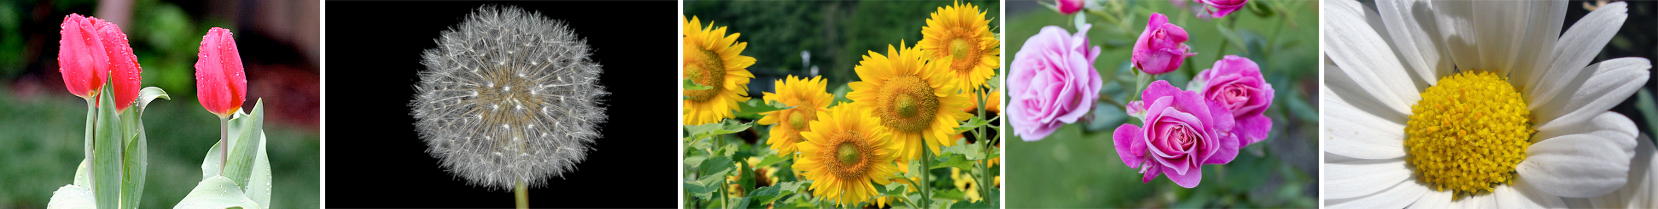
\includegraphics[width=0.8\textwidth]{img/flores}
\caption{Muestra del \textit{dataset} flores.}
\end{figure}

\item \textbf{\textit{ACDC}}: El \textit{dataset} \cite{acdcdataset} se compone de 150 pacientes reales de los que se les ha sacado unas resonancias magnéticas del corazón las cuales han sido anonimizadas. Las resonancias de los 150 pacientes están divididas en 5 clases (4 enfermedades y una normal). También incluye información adicional del paciente como el peso la altura, y los \textit{frames} claves de las resonancias. El \textit{dataset} pertenece a un reto (\textit{Automated Cardiac Diagnosis Challenge}) por eso solo se proporciona la segmentación de referencia de 100 pacientes las del resto son parte del reto. Las imágenes están en escala de grises y el formato es sin compresión. Las clases son: \textit{normal} (\textit{NOR}), \textit{myocardial infarction} (\textit{MINF}), \textit{dilated cardiomyopathy} (\textit{DCM}), \textit{hypertrophic cardiomyopathy} (\textit{HCM}) y \textit{abnormal right ventricle} (\textit{RV}).

\begin{figure}[H]
\centering
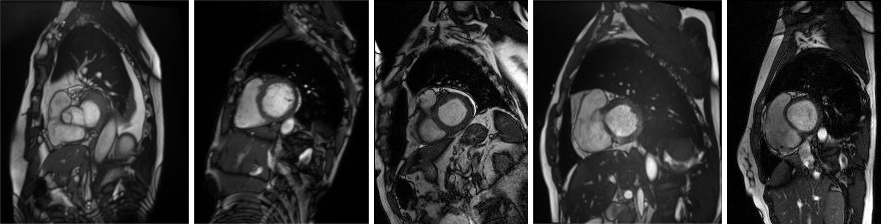
\includegraphics[width=0.8\textwidth]{img/acdc}
\caption{Muestra del \textit{dataset} \textit{ACDC}.}
\end{figure}

%TODO parrafo los datos ...

%TODO apartado imagenet

%TODO apartado cifar 10 100

\end{itemize}

%TODO apartado framework

\newpage
\section{Análisis de objetivos y metodología}
\subsection{Objetivos}
El objetivo principal de este trabajo es buscar una solución para la clasificación de enfermedades cardiacas en el \textit{dataset} \textit{ACDC} usando \textit{transfer learning} y diferentes enfoques para encontrar la solución que mejores resultados obtenga. Se usa como referencia el paper \textit{Automatic Segmentation and Disease Classification Using Cardiac Cine MR Images} ~\cite{DBLP:journals/corr/abs-1708-01141} en él proponen una solución en la que primero se segmentan las imágenes del corazón y luego se usa un clasificador \textit{random forest} para clasificar la imagen de entrada.
\bigskip

A diferencia del paper ~\cite{DBLP:journals/corr/abs-1708-01141} en el que se diseña una arquitectura específica y se entrena un modelo exclusivamente para ese problema, en este trabajo se parte de arquitecturas y modelos ya desarrollados y entrenados para resolver otro problema y se usa la técnica de \textit{transfer learning} para adaptarlo al nuevo problema.
\bigskip

El objetivo principal se divide en 4 objetivos más simples, para alcanzar el objetivo principal de forma más sencilla.

\begin{itemize}
\item \textbf{Objetivo 1}: Estudiar y analizar la forma en que se preprocesan y preparan los datos de entrada y el efecto que tienen en el rendimiento del modelo. También estudiar y analizar la preparación de un modelo para ser reentrenado.

\item \textbf{Objetivo 2}: Diseñar y probar diferentes enfoques y configuraciones de modelos, para mejorar la precisión de los resultados. Probar con \textit{datasets} de prueba y a continuación probar con el \textit{dataset} \textit{ACDC}.

\item \textbf{Objetivo 3}: Implementar \textit{scripts} en \textit{python} y \textit{bash} para probar los diferentes enfoques y configuraciones, usando el \textit{framework} \textit{TensorFlow}. Implementar \textit{scripts} para resumir y analizar la información.

\item \textbf{Objetivo 4}: Analizar y comparar los resultados de las diferentes pruebas, enfoques y configuraciones. Analizar los resultados obtenidos en las pruebas realizadas con los \textit{datasets} de prueba y en el \textit{dataset} \textit{ACDC}.
\end{itemize}

\subsection{Metodología}
La forma de realizar el trabajo es realizando distintas pruebas de diferentes características para estudiar cuál es la opción más interesante o que obtenga los mejores resultados.
\bigskip

Las pruebas se basan principalmente en el uso de redes neuronales como se describen en el apartado de ``Estado del arte’’, a las que se les aplica la técnica de \textit{transfer learning} para adaptar el modelo al problema que se quiere resolver. También se usan técnicas de distorsión de datos para mejorar la precisión y diferentes técnicas relacionadas con la organización de los modelos, como organizarlos en cascada.

\newpage
\section{Diseño y resolución del trabajo realizado}
En esta sección describo los pasos y las pruebas que he realizado y el proceso que he seguido para llegar a la solución que finalmente he obtenido, que consisten en realizar pruebas con diferentes modelos de partida ver los resultados obtenidos y analizar los resultados.
\bigskip

En estas pruebas todos los modelos de partida que he usado se han obtenido de la herramienta \textit{TensorFlow Hub}, los cuales ya vienen preparados para ser reentrenados para que solucionen otro problema. Todos los modelos han sido entrenados en el \textit{dataset} \textit{ImageNet} con 1000 clases, por lo tanto tienen el suficiente ``conocimiento'' como para resolver otro problema de clasificación menos exigente como por ejemplo la clasificación de 10 clases.

\subsection{Técnica bottleneck}
La técnica de \textit{bottleneck} consiste en obtener primero los valores del \textit{tensor} de salida de todos las imágenes de entrada, y guardar los valores, de esta manera no se tiene que ejecutar toda la red cada vez que vamos a entrenar con cierta imagen. De esta manera se entrena un modelo más pequeño, solamente las últimas capas y se usa como entrada de ese pequeño modelo la salida de toda la parte del modelo que no vamos a entrenar.
\bigskip

En cuanto a la inferencia usando esta técnica no cambia y se realiza de la misma manera que se haría con el resto de modelos que no usen esta técnica.

\begin{figure}[H]
\centering
\subfloat[Entrenamiento]{{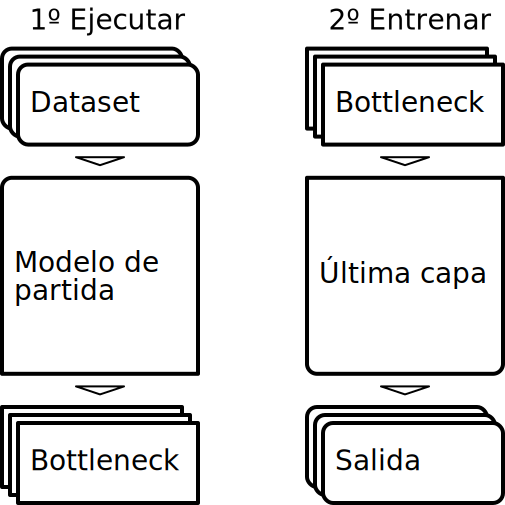
\includegraphics[valign=c, width=0.3\textwidth]{img/entrenamiento_bottleneck} }}%
\qquad
\subfloat[Inferencia]{{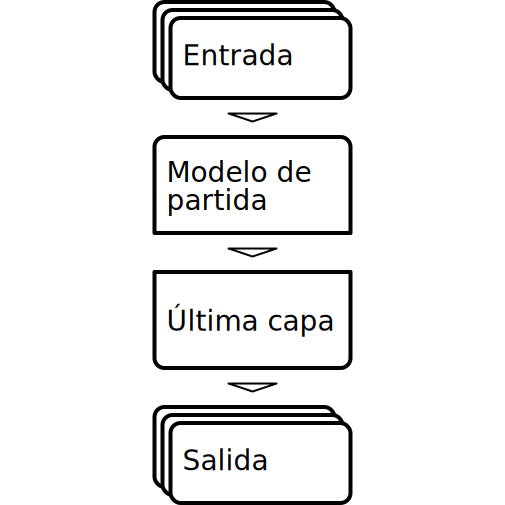
\includegraphics[valign=c, width=0.3\textwidth]{img/inferencia_bottleneck} }}%
\caption{Pasos para realizar el entrenamiento usando la técnica de \textit{bottleneck} y para la inferencia.}
\end{figure}

\subsection{Pruebas en otros datasets}
\subsubsection{Entrenamiento completo}
La primera prueba consiste en hacer un entrenamiento completo y así poder comparar los resultados con otras técnicas que voy a usar. En esta prueba se entrena de 0 la arquitectura \textit{AlexNet} para clasificar las imágenes del \textit{dataset} \textit{cifar 10}.

\begin{table}[H]
\centering
\begin{tabular}{|l|l|l|l|l|l|l|}
\hline
\textbf{Modelo} & \textbf{Dataset}              & \textbf{Clases}         & \textbf{Iteraciones}        & \textbf{Learning rate}   & \textbf{Batch size}      & \textbf{Precisión}        \\ \hline
AlexNet         & \multicolumn{1}{c|}{cifar 10} & \multicolumn{1}{c|}{10} & \multicolumn{1}{c|}{100000} & \multicolumn{1}{c|}{0.1} & \multicolumn{1}{c|}{128} & \multicolumn{1}{c|}{86.0} \\ \hline
\end{tabular}
\caption{Resultado entrenamiento completo.}
\end{table}

En esta prueba se obtiene un 86\% de precisión, que es un buen resultado para la prueba que se ha realizado, un entrenamiento completo. De esta forma se ha entrenado un modelo específicamente para ese \textit{dataset}.

\subsubsection{Añadir una capa totalmente conectada y softmax}
Esta prueba consiste en, a partir del modelo de partida eliminar la última capa y añadir una capa totalmente conectada y una capa de \textit{softmax}, esto se ha realizado con los \textit{datasets}: flores, \textit{cifar 10}, \textit{cifar 100} (20 clases) y \textit{cifar 100} (100 clases). El modelo de partida es \textit{inception v3}. Los resultados se pueden ver en la siguiente tabla:

\begin{table}[H]
\centering
\resizebox{\textwidth}{!}{%
\begin{tabular}{|l|l|c|c|c|c|c|}
\hline
\textbf{Modelo} & \textbf{Dataset}                                                  & \textbf{Clases} & \textbf{Iteraciones} & \textbf{Learning rate} & \textbf{Batch size} & \textbf{Precisión} \\ \hline
inception v3    & \begin{tabular}[c]{@{}l@{}}subconjunto\\ de cifar 10\end{tabular} & 3               & 4000                 & 0.01                   & 100                 & 93.8               \\ \hline
inception v3    & flores                                                            & 5               & 4000                 & 0.01                   & 100                 & 90.9               \\ \hline
inception v3    & cifar 10                                                          & 10              & 4000                 & 0.01                   & 100                 & 79.5               \\ \hline
inception v3    & cifar 100                                                         & 20              & 4000                 & 0.01                   & 100                 & 64.1               \\ \hline
inception v3    & cifar 100                                                         & 100             & 4000                 & 0.01                   & 100                 & 51.7               \\ \hline
\end{tabular}%
}
\caption{Resultados añadir una capa totalmente conectada y \textit{softmax}.}
\end{table}

En la tabla se puede ver que cuantas más clases se requiera identificar menos precisión se obtiene, esto se debe a que el problema a resolver es más difícil.
\bigskip

A continuación se hace la misma prueba pero usando como modelo de partida \textit{resnet v2 152} que es un modelo basado también en convoluciones pero de mayor tamaño.

\begin{table}[H]
\centering
\resizebox{\textwidth}{!}{%
\begin{tabular}{|l|l|c|c|c|c|c|}
\hline
\textbf{Modelo} & \textbf{Dataset}                                                  & \textbf{Clases} & \textbf{Iteraciones} & \textbf{Learning rate} & \textbf{Batch size} & \textbf{Precisión} \\ \hline
resnet v2 152   & \begin{tabular}[c]{@{}l@{}}subconjunto\\ de cifar 10\end{tabular} & 3               & 4000                 & 0.01                   & 100                 & 94.4               \\ \hline
resnet v2 152   & cifar 10                                                          & 10              & 40000                & 0.01                   & 100                 & 82.9               \\ \hline
resnet v2 152   & cifar 100                                                         & 20              & 14000                & 0.01                   & 100                 & 70.8               \\ \hline
\end{tabular}%
}
\caption{Resultados prueba usando modelo basado en la arquitectura \textit{resnet v2 512}.}
\end{table}

En los resultados de estas pruebas podemos observar que para el mismo número de clases se obtienen unos resultados ligeramente mejores, esto se debe a que la información a la salida del modelo de partida es más significativa ya que a pasado por más capas, por lo tanto la información de entrada ha sido más procesada.
\bigskip

En comparación, el resultado del entrenamiento completo, para la prueba equivalente (10 clases, 86.0\% entrenamiento completo, 82.9\% \textit{transfer learning}), es ligeramente mejor que con la técnica de \textit{transfer learning}. El resultado de la prueba del entrenamiento completo es mejor porque en ese caso se está entrenando el modelo por completo y de esa forma se consigue un modelo específico para ese \textit{dataset}, al contrario que con \textit{transfer learning} en el que se parte de un modelo ya entrenado en otro \textit{dataset} y solo se entrenan las últimas capas con el nuevo \textit{dataset}.
\bigskip

Esto tiene sus ventajas y desventajas, por un lado entrenar un modelo completo requiere más recursos pero se pueden obtener mejores resultados, sin embargo en \textit{transfer learning} los recursos necesarios son menos y se puede obtener resultados parecidos.
\bigskip

Para esta prueba se ha usado el \textit{script} \texttt{retrain.py} ~\cite{retrainpy}, el cual hace uso de la técnica de \textit{bottleneck} y de la herramienta \textit{TensorFlow Hub}.
\bigskip

Para cargar un modelo de \textit{TensorFlow Hub} se hace de la siguiente forma:

\begin{lstlisting}[language=Python]
module_spec = hub.load_module_spec(module_url)
input_tensor = tf.placeholder(tf.float32, [None, height, width, 3])
m = hub.Module(module_spec)
output_tensor = m(input_tensor)
\end{lstlisting}

Donde \texttt{module\_url} es la \textit{url} del módulo que se quiere cargar, los modelos disponibles se pueden encontrar en la pagina \url{https://tfhub.dev} e \texttt{input\_tensor} y \texttt{output\_tensor} son referencias a los tensores de entrada y salida respectivamente.
\bigskip

Una vez cargado el modelo se puede añadir la última capa y la función de optimización.

\begin{lstlisting}[language=Python]
# tensores de entrada
bottleneck_input = tf.placeholder_with_default(output_tensor,
  shape=[batch_size, bottleneck_tensor_size],)
ground_truth_input = tf.placeholder(tf.int64, [batch_size])

# añadir una capa totalmente conectada y softmax
layer_weights = tf.Variable(initial_value)
layer_biases = tf.Variable(tf.zeros([bottleneck_tensor_size]))
logits = tf.matmul(bottleneck_input, layer_weights) + layer_biases
final_tensor = tf.nn.softmax(logits)

# añadir funcion de error y operaciones de optimizacion
cross_entropy_mean = tf.losses.sparse_softmax_cross_entropy(
  labels=ground_truth_input, logits=logits)
optimizer = tf.train.GradientDescentOptimizer(learning_rate)
train_step = optimizer.minimize(cross_entropy_mean)
\end{lstlisting}

Por último para ejecutar una iteración del entrenamiento se hace de la siguiente forma.

\begin{lstlisting}[language=Python]
sess.run(train_step,
  feed_dict={bottleneck_input: train_bottlenecks,
             ground_truth_input: train_ground_truth})
\end{lstlisting}

Donde \texttt{train\_step} es el último nodo del grafo que se ha construido, y por lo tanto para ejecutar ese nodo se ejecutará todo el grafo que depende de él, que hará que se ejecute una iteración. \texttt{train\_bottlenecks} y \texttt{train\_ground\_truth} son las entrada del conjunto de datos y las clases correctas para cada clase del \textit{batch} que se está ejecutando respectivamente.

\subsubsection{Añadir 3 capas totalmente conectadas}
En esta prueba al modelo de partida se le añaden tres capas totalmente conectadas, los resultados son los siguientes:

\begin{table}[H]
\centering
\resizebox{\textwidth}{!}{%
\begin{tabular}{|l|l|c|c|c|c|c|}
\hline
\textbf{Modelo} & \textbf{Dataset} & \textbf{Clases} & \textbf{Iteraciones} & \textbf{Learning rate} & \textbf{Batch size} & \textbf{Precisión} \\ \hline
inception v3    & cifar 10         & 10              & 4000                 & 0.01                   & 100                 & 34.1               \\ \hline
inception v3    & cifar 10         & 10              & 50000                & 0.01                   & 100                 & 79.9               \\ \hline
inception v3    & cifar 100        & 100             & 60000                & 0.01                   & 100                 & 45.5               \\ \hline
\end{tabular}%
}
\caption{Resultados añadir 3 capas totalmente conectadas.}
\end{table}

En estos resultados podemos ver que al poner más capas, especialmente capas totalmente conectadas, el entrenamiento requiere más iteraciones (en la primera prueba el modelo no llegó a converger en la configuración más óptima), y por lo tanto más tiempo para obtener los mismos resultados que con una capa. También podemos ver que los resultados son similares o incluso ligeramente peores que solo con una capa totalmente conectada.
\bigskip

En esta prueba se ha modificado el \textit{script} \texttt{retrain.py} para añadir 3 capas totalmente conectadas:

\begin{lstlisting}[language=Python]
# tensores de entrada
bottleneck_input = tf.placeholder_with_default(
    output_tensor,
    shape=output_tensor.get_shape())
ground_truth_input = tf.placeholder(
    tf.int64, [batch_size])

# añadir tres capas totalmente conectada y softmax
# layer0
with tf.name_scope('final_retrain_ops0'):
    layer_weights = tf.Variable(initial_value)
    layer_biases = tf.Variable(tf.zeros([bottleneck_tensor_size]))
    logits = tf.matmul(bottleneck_input, layer_weights) + layer_biases

# layer1
with tf.name_scope('final_retrain_ops1'):
    layer_weights = tf.Variable(initial_value)
    layer_biases = tf.Variable(tf.zeros([bottleneck_tensor_size]))
    logits = tf.matmul(logits, layer_weights) + layer_biases

# layer 2
with tf.name_scope('final_retrain_ops'):
    layer_weights = tf.Variable(initial_value)
    layer_biases = tf.Variable(tf.zeros([class_count]))
    logits = tf.matmul(logits, layer_weights) + layer_biases

final_tensor = tf.nn.softmax(logits)

# añadir funcion de error y operaciones de optimizacion
cross_entropy_mean = tf.losses.sparse_softmax_cross_entropy(
    labels=ground_truth_input, logits=logits)
optimizer = tf.train.GradientDescentOptimizer(learning_rate)
train_step = optimizer.minimize(cross_entropy_mean)
\end{lstlisting}


\subsubsection{Quitar 2 capas}
Esta prueba consiste en, del modelo de partida en vez de quitarle una capa quitarle más capas y ver que pasa. En este caso quito dos capas y añado una capa de \textit{average pool} y a continuación añadir tres capas totalmente conectadas. La capa \textit{average pool} la añado para reducir los valores en una dimensión, el \textit{tensor} pasa de ser de dos dimensiones a una. Los resultados son los siguientes:

\begin{table}[H]
\centering
\resizebox{\textwidth}{!}{%
\begin{tabular}{|l|l|c|c|c|c|c|}
\hline
\textbf{Modelo} & \textbf{Dataset}                                                  & \textbf{Clases} & \textbf{Iteraciones} & \textbf{Learning rate} & \textbf{Batch size} & \textbf{Precisión} \\ \hline
inception v3    & cifar 10                                                          & 10              & 100000               & 0.01                   & 100                 & 79.8               \\ \hline
inception v3    & \begin{tabular}[c]{@{}l@{}}subconjunto\\ de cifar 10\end{tabular} & 3               & 70000                & 0.01                   & 100                 & 95.5               \\ \hline
\end{tabular}%
}
\caption{Resultados quitar 2 capas.}
\end{table}

En estas pruebas se puede ver que no se obtienen diferencias en cuanto a la precisión, quitar dos capas no ha producido ningún resultado notablemente distinto. Mediante esta prueba se puede deducir que el modelo de partida es tan grande que aunque le quitemos dos capas sigue teniendo el mismo rendimiento, la capa que se ha quitado se puede pensar como redundante y no comprimía la información más de lo que ya estaba.
\bigskip

Para esta prueba se ha modificado el \textit{script} \texttt{retrain.py}, para que acepte un parámetro en el que se le especifique la capa desde la que se quiere reentrenar. Para especificar la capa se a modificado la parte de donde se hace la carga del modelo:

\begin{lstlisting}[language=Python]
module_spec = hub.load_module_spec(module_url)
input_tensor = tf.placeholder(tf.float32, [None, height, width, 3])
m = hub.Module(module_spec)
outputs = m(input_tensor, signature=model_signature, as_dict=True)
output_tensor = outputs[retrain_from_layer]
\end{lstlisting}

Al quitar más capas es posible que se de la situación de que la capa de salida del modelo de partida tenga más dimensiones, por lo que antes de añadir la última capa se añade también una capa de \textit{pooling} para reducir una dimensión:

\begin{lstlisting}[language=Python]
# tensores de entrada
bottleneck_input = tf.placeholder_with_default(
    output_tensor,
    shape=output_tensor.get_shape())

bottleneck_input = tf.nn.avg_pool(bottleneck_input)
bottleneck_input = tf.reshape(bottleneck_input)
\end{lstlisting}


\subsubsection{Quitar 3 capas}
Esta prueba consiste en, del modelo de partida en vez de quitarle una capa quitarle más capas y ver que pasa. En este caso quito tres capas y añado una capa de \textit{average pool} y a continuación añadir tres capas totalmente conectadas. La capa \textit{average pool} la añado para reducir los valores en una dimensión, el \textit{tensor} pasa de ser de dos dimensiones a una. Los resultados son los siguientes:

\begin{table}[H]
\centering
\resizebox{\textwidth}{!}{%
\begin{tabular}{|l|l|c|c|c|c|c|}
\hline
\textbf{Modelo} & \textbf{Dataset}                                                  & \textbf{Clases} & \textbf{Iteraciones} & \textbf{Learning rate} & \textbf{Batch size} & \textbf{Precisión} \\ \hline
inception v3    & cifar 10                                                          & 10              & 90000                & 0.01                   & 100                 & 56.0               \\ \hline
inception v3    & \begin{tabular}[c]{@{}l@{}}subconjunto\\ de cifar 10\end{tabular} & 3               & 70000                & 0.01                   & 100                 & 95.9               \\ \hline
\end{tabular}%
}
\caption{Resultados quitar 3 capas.}
\end{table}

En este caso, al contrario que en el anterior sí que se puede observar una degradación de la precisión en el resultado, en el caso del problema de tres clases sigue obteniendo un resultado parecido pero en el problema de diez clases si se puede apreciar un importante pérdida de precisión.
\bigskip

Para esta prueba se ha usado el mismo \textit{script} que en el apartado anterior pero con otros parámetros.

\subsection{Pruebas en el dataset ACDC}
A continuación detallo las diferentes pruebas realizadas sobre el dataset \textit{ACDC} y analizo los resultados obtenidos.

\subsubsection{Añadir una capa}
La primera idea consiste en a partir del \textit{dataset} extraer todos los \textit{slices} de todos los pacientes y de todo ese conjunto de imágenes dividirlas en los sets de entrenamiento, validación y test. En cuanto al modelo se usa \textit{inception v3} de partida y se le añade una capa totalmente conectada al final. El resultado obtenido es el siguiente:

\begin{table}[H]
\centering
\begin{tabular}{|l|c|c|c|c|c|}
\hline
\textbf{Prueba} & \textbf{Modelo} & \textbf{Clases} & \textbf{Iteraciones} & \textbf{Learning rate} & \textbf{Precisión} \\ \hline
Añadir una capa & inception v3    & 5               & 4000                 & 0.01                   & 99.5               \\ \hline
\end{tabular}
\caption{Resultado añadir una capa.}
\end{table}

El resultado parece augurar que con esta primera prueba ya he solucionado el problema, pero la realidad es que la forma en la que se ha repartido el \textit{dataset} ha originado \textit{overfitting}. El reparto del \textit{dataset} en los conjuntos de entrenamiento, validación y test ha hecho que sea posible que en los tres conjuntos haya imágenes de cualquier paciente por lo que la red realmente no estaba aprendiendo a clasificar las enfermedades sino a recordar que paciente del \textit{dataset} tiene que enfermedad.
\bigskip

El efecto de esto es que cuando se hace la inferencia sobre imágenes de los pacientes que están en el \textit{dataset}, aunque realmente esa imagen no haya sido usada en el entrenamiento, el modelo funcionará. Pero si se hace la inferencia sobre imágenes de otro paciente totalmente nuevo para este modelo probablemente no funcione bien. En la siguiente sección explicaré cómo solucionar el problema del \textit{overfitting} que he tenido en esta prueba.
\bigskip

Para esta prueba se ha implementado el script \texttt{acdc\_nii\_to\_jpg.py} que lee los ficheros \texttt{nii}, los extrae, guarda las imágenes en formato \texttt{jpg} y organiza en carpetas según la clase de la imagen para preparar las imágenes para ser usadas en el script \texttt{retrain.py}. Se usa el \textit{script} \texttt{retrain.py} para hacer el \textit{transfer learning}. Y se ha implementado el \textit{script} \texttt{batch\_inference.py} (basado en \texttt{retrain.py}) para evaluar el resultado del modelo entrenado, este \textit{script} hace uso de la \textit{api} de \textit{TensorFlow} \texttt{saved\_model} para cargar el modelo entrenado en el \textit{script} \texttt{retrain.py} y hacer la inferencia en el conjunto de test.
\bigskip

En el \textit{script} \texttt{batch\_inference.py}, para cargar un modelo se usa el siguiente código:

\begin{lstlisting}[language=Python]
    tf.saved_model.loader.load(
      sess,
      [tag_constants.SERVING],
      FLAGS.saved_model_dir
    )
\end{lstlisting}

Donde \texttt{FLAGS.saved\_model\_dir} es la carpeta donde está guardado el modelo.
\bigskip

Y para hacer la inferencia se hace la siguiente llamada con cada una de las imágenes del conjunto de test para ejecutar el modelo que da como salida la clase que se ha predicho.

\begin{lstlisting}[language=Python]
          result = sess.run(prediction,
                            {image: resized_image})
\end{lstlisting}

Donde \texttt{image} es el \textit{tensor} de entrada del modelo, \texttt{prediction} es el \textit{tensor} de salida del modelo y \texttt{resized\_image} es un \textit{array} con la imagen de entrada descodificada y con el tamaño de entrada del modelo. La salida del modelo es almacenada en \texttt{result} como un \textit{array} de probabilidades entre 0 y 1, con tantas posiciones como clases hay, la posición que tenga mayor valor será la clase predicha.
\bigskip

En el \textit{script} \texttt{acdc\_test.sh} se llaman a los \textit{scripts} anteriores donde se pueden ver los parámetros usados para el entrenamiento del modelo.

\begin{lstlisting}[language=Bash]
python retrain.py \
  --image_dir="datasets/acdc/" \
  --output_graph="$results_dir/output_graph.pb" \
  --output_labels="$results_dir/output_labels.txt" \
  --summaries_dir="$results_dir/retrain_logs" \
  --how_many_training_steps=4000 \
  --learning_rate=0.01 \
  --testing_percentage=10 \
  --validation_percentage=10 \
  --eval_step_interval=10 \
  --train_batch_size=100 \
  --test_batch_size=-1 \
  --validation_batch_size=100 \
  --bottleneck_dir="output/01_acdc_test/bottleneck" \
  --final_tensor_name="final_result" \
  --tfhub_module="https://tfhub.dev/google/imagenet/inception_v3/feature_vector/3" \
  --saved_model_dir="$results_dir/saved_model/" \
  --checkpoint_path="$results_dir/_retrain_checkpoint" 2>&1 | tee "$results_dir/output_retrain"


python batch_inference.py \
  --image_dir="datasets/acdc/" \
  --set testing \
  --saved_model_dir="$results_dir/saved_model/" \
  --output_labels="$results_dir/output_labels.txt" \
  --output_predictions="$results_dir/output_predictions.csv" \
  --testing_percentage=10 \
  --validation_percentage=10 \
  --tfhub_module="https://tfhub.dev/google/imagenet/inception_v3/feature_vector/3" 2>&1 | tee "$results_dir/output_inference"
\end{lstlisting}

\subsubsection{Repartir bien los sets}
Esta prueba es básicamente lo mismo que la anterior en cuanto al modelo, pero teniendo en cuenta que los sets de entrenamiento, validación y test deben de estar repartidos por paciente. Es decir todos las imágenes de un paciente deben de ir al mismo set y no se pueden encontrar en más de un set imágenes del mismo paciente. De esta forma se evita que haya imágenes relacionadas en sets distintos y por lo tanto no se pueda saber la enfermedad relacionándolas.
\bigskip

También se tiene en cuenta que todas las clases deben de estar representadas por igual en todos los sets, es decir no debe de haber una diferencia muy grande entre la cantidad de pacientes en cada set, de lo contrario se podría generar \textit{overfitting} porque hay más imágenes de una clase que harían que el modelo tendiese a dar más resultados de la clase que más imágenes tiene simplemente porque aparece más.

\begin{table}[H]
\centering
\begin{tabular}{|l|c|c|c|c|c|}
\hline
\textbf{Prueba} & \textbf{Modelo} & \textbf{Clases} & \textbf{Iteraciones} & \textbf{Learning rate} & \textbf{Precisión} \\ \hline
Añadir una capa & inception v3    & 5               & 4000                 & 0.01                   & 63.2               \\ \hline
\end{tabular}
\caption{Resultado repartir bien los sets.}
\end{table}

En este caso se obtiene un resultado más realista ya que las imágenes del set de test no están relacionadas con las del entrenamiento ni las de validación. En las siguientes secciones explicaré otras técnicas que he usado para enfocar el problema de clasificar los pacientes de forma que se puede obtener una mejor precisión. Desde esta prueba y en adelante el reparto de los sets se hará como en esta prueba para no volver a tener el problema del \textit{overfitting}.
\bigskip

En esta prueba los \textit{scripts} son los mismos que en la anterior pero el \textit{script} \texttt{acdc\_nii\_to\_jpg.py} ha sido modificado para que en el nombre de los ficheros añada ``\texttt{\_nohash\_}'' después del índice de paciente para que a la hora de hacer la repartición de los conjuntos de entrenamiento en el \textit{scritp} \texttt{retrain.py} todos los pacientes vayan al mismo conjunto. De forma que el nombre de un fichero pasa de ser así: \texttt{patient001\_frame00\_slice00.jpg} a ser así: \texttt{patient001\_nohash\_frame00\_slice00.jpg}.
\bigskip

El \textit{script} \texttt{retrain.py} usa una función de dispersión para repartir de forma aleatoria las imágenes del \textit{dataset} de entrada en los conjuntos de entrenamiento. A la función de dispersión se le pasa como entrada el nombre del fichero quitándole lo que tenga después de la cadena ``\texttt{\_nohash\_}’’ en el nombre del fichero. La salida de la función de dispersión se usa para determinar en qué conjunto se incluye la imagen.

\begin{lstlisting}[language=Python]
base_name = os.path.basename(file_name)
name = re.sub(r'_nohash_.*$', '', file_name)
hash = hashlib.sha1(tf.compat.as_bytes(name)).hexdigest()
percentage = ((int(hash, 16) % (MAX + 1)) * (100.0 / MAX))
if percentage < validation_percentage:
  validation_images.append(base_name)
elif percentage < (testing_percentage + validation_percentage):
  testing_images.append(base_name)
else:
  training_images.append(base_name)
\end{lstlisting}

De esta forma para todas las imágenes de un mismo paciente se le pasará como entrada a la función de dispersión los mismos datos que harán que el resultado de la función sea el mismo para todas las imágenes del mismo paciente y por lo tanto incluyendo todas sus imágenes en el mismo conjunto.

\subsubsection{Usar un slice por paciente}
En esta prueba en vez de usar todas las imágenes de todos los pacientes se usa solo una imagen de cada paciente, de esta forma se pretende reducir el \textit{overfitting} que hay en el modelo al haber muchas imágenes relacionadas de cada paciente, que hace que el modelo converja a algo que no se está buscando. En esta prueba uso solamente el primer \textit{slice} del primer \textit{frame} de cada paciente.

\begin{table}[H]
\centering
\begin{tabular}{|l|l|l|l|l|l|}
\hline
\textbf{Prueba}                                                      & \textbf{Modelo}                   & \textbf{Clases}        & \textbf{Iteraciones}      & \textbf{Learning rate}    & \textbf{Precisión}        \\ \hline
\begin{tabular}[c]{@{}l@{}}Usar un slice\\ por paciente\end{tabular} & \multicolumn{1}{c|}{inception v3} & \multicolumn{1}{c|}{5} & \multicolumn{1}{c|}{4000} & \multicolumn{1}{c|}{0.01} & \multicolumn{1}{c|}{42.9} \\ \hline
\end{tabular}
\caption{Resultado usar un \textit{slice} por paciente.}
\end{table}

En esta prueba el resultado obtenido es un 42\% de precisión que es bastante malo, por lo que esta prueba no ha tenido éxito. Esto puede deberse a que si se cojo únicamente un \textit{slice} por paciente el tamaño del \textit{dataset} de entrada se reduce considerablemente y puede que no haya suficientes muestras para poder hacer un entrenamiento lo suficientemente bueno.
\bigskip

Para esta prueba se usan los \textit{scripts} \texttt{acdc\_one\_slice\_retrain.py} y \\ \texttt{acdc\_one\_slice\_batch\_inference.py} que parten de los \textit{scripts} del apartado anterior para que filtren las imágenes de entrada y solo usen una imagen por paciente. A los \textit{script} anteriores se les han añadido la siguiente línea:

\begin{lstlisting}[language=Python]
file_glob = os.path.join(image_dir, dir_name, '*frame00_slice00.' + extension)
\end{lstlisting}

En el \textit{script} \texttt{acdc\_one\_slice\_test.sh} se llaman a los \textit{scripts} anteriores donde se pueden ver los parámetros usados para el entrenamiento del modelo.

\subsubsection{Entrenamiento por subsets}
La idea consiste en agrupar las clases en varios grupos de esta forma reducir el número de posibilidades entre las que tiene que diferenciar el modelo.
\bigskip

A continuación se muestran los resultados obtenidos de agrupar las clases de la siguiente manera: se hacen dos grupos uno con una clase por separado en un grupo y el resto de clases en otro grupo, esta forma de agrupar las clases también se puede ver como un modelo que te diga si cierta imagen pertenece a una clase o no.

\begin{table}[H]
\centering
\resizebox{\textwidth}{!}{%
\begin{tabular}{|l|c|l|c|c|c|}
\hline
\textbf{Prueba}                                                              & \textbf{Modelo}                                        & \multicolumn{1}{c|}{\textbf{Subsets de clases}}                & \textbf{Iteraciones} & \textbf{\begin{tabular}[c]{@{}c@{}}Learning\\ rate\end{tabular}} & \textbf{Precisión} \\ \hline
\begin{tabular}[c]{@{}l@{}}Entrenamiento\\ por subsets\\ (DCM)\end{tabular}  & \begin{tabular}[c]{@{}c@{}}inception\\ v3\end{tabular} & \begin{tabular}[c]{@{}l@{}}DCM:\\ HCM,MINF,NOR,RV\end{tabular} & 4000                 & 0.01                                                             & 83.9               \\ \hline
\begin{tabular}[c]{@{}l@{}}Entrenamiento\\ por subsets\\ (HCM)\end{tabular}  & \begin{tabular}[c]{@{}c@{}}inception\\ v3\end{tabular} & \begin{tabular}[c]{@{}l@{}}HCM:\\ DCM,MINF,NOR,RV\end{tabular} & 4000                 & 0.01                                                             & 76.5               \\ \hline
\begin{tabular}[c]{@{}l@{}}Entrenamiento\\ por subsets\\ (MINF)\end{tabular} & \begin{tabular}[c]{@{}c@{}}inception\\ v3\end{tabular} & \begin{tabular}[c]{@{}l@{}}MINF:\\ DCM,HCM,NOR,RV\end{tabular} & 4000                 & 0.01                                                             & 81.6               \\ \hline
\begin{tabular}[c]{@{}l@{}}Entrenamiento\\ por subsets\\ (NOR)\end{tabular}  & \begin{tabular}[c]{@{}c@{}}inception\\ v3\end{tabular} & \begin{tabular}[c]{@{}l@{}}NOR:\\ DCM,HCM,MINF,RV\end{tabular} & 4000                 & 0.01                                                             & 89.8               \\ \hline
\begin{tabular}[c]{@{}l@{}}Entrenamiento\\ por subsets\\ (RV)\end{tabular}   & \begin{tabular}[c]{@{}c@{}}inception\\ v3\end{tabular} & \begin{tabular}[c]{@{}l@{}}RV:\\ DCM,HCM,MINF,NOR\end{tabular} & 4000                 & 0.01                                                             & 85.8               \\ \hline
\end{tabular}%
}
\caption{Resultados entrenamientos por subsets. Nota: en la columna ``Subsets de clases'', ``:'' indican la separación de subsets.}
\end{table}

Como se puede ver la precisión aumenta ya que el problema a resolver se ha simplificado, ha pasado de tener que resolver un problema de clasificar 5 clases a tener que clasificar 2 grupos.
\bigskip

Esta idea no se puede considerar una idea completa porque realmente se han entrenado 5 modelos y cada uno da una salida. Cada uno de estos modelos da una salida que te dice si la imagen de la entrada pertenece a una clase o al resto. Hay 5 modelos uno por cada clase y cada uno de ellos te dice si la imagen de entrada pertenece a esa clase. En el caso de que quisiéramos usarlo, por ejemplo haciendo la inferencia en estos 5 modelos, se puede dar una situación en la que sí podría dar una solución pero otras dos situaciones en las que daría una respuesta sin solución.
\bigskip

De esta forma si tenemos un modelo por cada clase y cada modelo te dice si la entrada es esa clase o no. La mejor situación que se puede presentar es que solo uno de estos modelos diga que la imagen de entrada sea la clase del modelo y la respuesta del resto de modelos sea que la clase pertenece al resto de modelos. En la siguiente tabla se puede ver un ejemplo de ejecución de los cinco modelos en la que se da una situación favorable.

\begin{table}[H]
\centering
\resizebox{\textwidth}{!}{%
\begin{tabular}{|c|c|c|c|c|c|}
\hline
                                           & \textbf{\begin{tabular}[c]{@{}c@{}}Modelo\\ DCM\end{tabular}} & \textbf{\begin{tabular}[c]{@{}c@{}}Modelo\\ HCM\end{tabular}} & \textbf{\begin{tabular}[c]{@{}c@{}}Modelo\\ MINF\end{tabular}} & \textbf{\begin{tabular}[c]{@{}c@{}}Modelo\\ NOR\end{tabular}} & \textbf{\begin{tabular}[c]{@{}c@{}}Modelo\\ RV\end{tabular}} \\ \hline
\textbf{¿Pertenece a la clase del modelo?} & Sí                                                            & No                                                            & No                                                             & No                                                            & No                                                           \\ \hline
\textbf{¿Pertenece al resto de clases?}    & No                                                            & Sí                                                            & Sí                                                             & Sí                                                            & Sí                                                           \\ \hline
\end{tabular}%
}
\caption{Ejemplo situación favorable.}
\end{table}

Las dos situaciones en las que no se puede dar una solución, son que ningún de estos modelos diga que la imagen de entrada es la clase del modelo o que más de uno de estos modelos diga que la imagen de entrada es la clase del modelo. En la siguiente tabla se pueden ver dos ejemplos de ejecución de los cinco modelos en los que se dan las dos situaciones en las que no se puede dar una solución.

\begin{table}[H]
\centering
\resizebox{\textwidth}{!}{%
\begin{tabular}{|c|c|c|c|c|c|c|c|c|c|c|}
\hline
                                                                                     & \multicolumn{5}{c|}{\textbf{Situación 1}}                                                                                                                                                                                                                                                                                     & \multicolumn{5}{c|}{\textbf{Situación 2}}                                                                                                                                                                                                                                                                                     \\ \hline
                                                                                     & \textbf{\begin{tabular}[c]{@{}c@{}}Modelo\\ DCM\end{tabular}} & \textbf{\begin{tabular}[c]{@{}c@{}}Modelo\\ HCM\end{tabular}} & \textbf{\begin{tabular}[c]{@{}c@{}}Modelo\\ MINF\end{tabular}} & \textbf{\begin{tabular}[c]{@{}c@{}}Modelo\\ NOR\end{tabular}} & \textbf{\begin{tabular}[c]{@{}c@{}}Modelo\\ RV\end{tabular}} & \textbf{\begin{tabular}[c]{@{}c@{}}Modelo\\ DCM\end{tabular}} & \textbf{\begin{tabular}[c]{@{}c@{}}Modelo\\ HCM\end{tabular}} & \textbf{\begin{tabular}[c]{@{}c@{}}Modelo\\ MINF\end{tabular}} & \textbf{\begin{tabular}[c]{@{}c@{}}Modelo\\ NOR\end{tabular}} & \textbf{\begin{tabular}[c]{@{}c@{}}Modelo\\ RV\end{tabular}} \\ \hline
\textbf{\begin{tabular}[c]{@{}c@{}}¿Pertenece a la\\ clase del modelo?\end{tabular}} & Sí                                                            & Sí                                                            & No                                                             & No                                                            & No                                                           & No                                                            & No                                                            & No                                                             & No                                                            & No                                                           \\ \hline
\textbf{\begin{tabular}[c]{@{}c@{}}¿Pertenece al\\ resto de clases?\end{tabular}}    & No                                                            & No                                                            & Sí                                                             & Sí                                                            & Sí                                                           & Sí                                                            & Sí                                                            & Sí                                                             & Sí                                                            & Sí                                                           \\ \hline
\end{tabular}%
}
\caption{Ejemplo situación en la que no se puede dar una solución.}
\end{table}

Esta idea se usa como base para hacer la siguiente prueba.
\bigskip

Para esta prueba se ha modificado el \textit{script} \texttt{retrian.py} para que acepte un parámetro en el que se le puede especificar cómo se organizan los subsets. El \textit{script} para ejecutar el entrenamiento de esta prueba es \texttt{acdc\_subset\_retrain.py}. En concreto en el método \texttt{create\_image\_lists()} se ha modificado para que reparta los conjuntos de entrenamiento según se especifica en el parámetro.

\begin{lstlisting}[language=Python]
def create_image_lists(image_dir, subsets, testing_percentage, validation_percentage):
  (...)
  subsets_list = []
  for subset in subsets.split(":"):
    subset_list = []
    for sub_dir in subset.split(","):
      subset_list.append(sub_dir)
    subsets_list.append(subset_list)

  for subset_list in subsets_list:
    label_name = "_".join([re.sub(r'[^a-z0-9]+', ' ', dir_name.lower()) for dir_name in subset_list])
    (...)
    training_images = []
    for dir_name in subset_list:
      file_list = []
      file_glob = os.path.join(image_dir, dir_name, '*')
      file_list.extend(tf.gfile.Glob(file_glob))
      (...)
      for file_name in file_list:
        base_name = os.path.basename(file_name)
        base_name = os.path.join(dir_name, base_name)
        (...)
        training_images.append(base_name)
    result[label_name] = {
        'training': training_images,
    }
  return result
\end{lstlisting}

Para hacer la inferencia se usa el \textit{script} \texttt{acdc\_subset\_batch\_inference.py} que es una modificación del \textit{script} \texttt{batch\_inference.py} que también incorpara los cambios descritos anteriormente.

En el \textit{script} \texttt{acdc\_subset\_test.sh} se llaman a los \textit{scripts} anteriores donde se pueden ver los parámetros usados para el entrenamiento de cada modelo. En este caso se entrenan cinco modelos, uno por cada clase.

\subsubsection{Cascada}
Esta idea consiste en partiendo de la idea anterior hacer modelos que vayan identificando o descartando enfermedades cada uno una. Los cuales se ejecutan en secuencia uno tras otro, cada uno teniendo solo que identificar entre dos grupos de clases. De esta forma se pretende mejorar la precisión final simplificando el problema para cada uno de los modelos. Cada modelo solo tiene que decir si una imagen pertenece o no a una clase.

\begin{itemize}

\item \textbf{Entrenamineto}: El entrenamiento de los modelos se hace por pasos, primero se entrena un modelo por cada clase que hay en el \textit{dataset}. Los modelos se entrenan usando la idea del apartado anterior y las clases se dividen en la clase a la que el modelo hace referencia y el resto. Con estos modelos lo que se pretende es decir si la imagen de entrada pertenece a la clase a la que hace referencia el modelo o no. Al final del primer paso se acaba con tantos modelos como clases haya, cada uno haciendo referencia a una clase que la identifica o la descarta.
\bigskip

De los modelos del paso anterior se escoge el que mas precision haya obtenido, se elimina del conjunto de clases la clase a la que hace referencia el modelo que se ha escogido y se repite el paso anterior con las clases que quedan hasta que queden solo dos clases.
\bigskip

Por último cuando ya solo quedan dos clases ya no se entrena un modelo por cada clase que queda, no tiene sentido ya que la clase a la que hace referencia el modelo sería una y en el grupo de otros solo quedaría una y viceversa. Es decir cuando ya solo quedan dos clases solo se entrena un modelo que dice si es una clase u otra.

\begin{figure}[H]
\centering
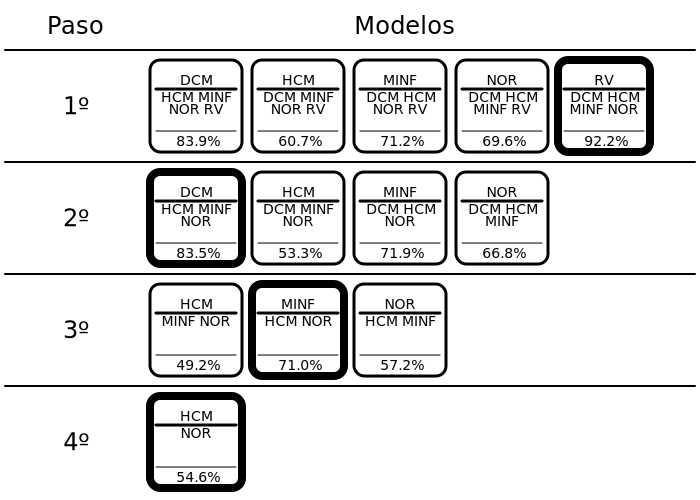
\includegraphics[width=0.6\textwidth]{img/entrenamiento_cascada}
\caption{Entrenamiento cascada.}
\end{figure}

\item \textbf{Inferencia}: Al final del entrenamiento de todos los modelos se acaba con unos modelos de los cuales solo se usan los que hayan obtenido los mejores resultados en cada paso, el resto ya no son necesarios. Los modelos de cada paso que se escogen son el modelo del paso, cada uno. La inferencia se hace siguiendo los siguientes pasos:

\begin{itemize}
\item Se hace la inferencia en el modelo del primer paso en el que se identifica o se descarta una enfermedad.

\item Si en el paso anterior se identifica la enfermedad, la inferencia termina y el resultado es la clase que se ha identificado en el paso anterior, si la clase del paso anterior se ha descartado se continúa con el modelo del siguiente paso, que igualmente identifica o descarta una clase. Esto se repite con todos los pasos hasta el último paso.

\item En el último paso ya no se identifica o se descarta una clase porque el último paso solo queda identificar dos clases. Si se llega a este paso entonces el resultado de la inferencia es el resultado de este último modelo.
\end{itemize}

\begin{figure}[H]
\centering
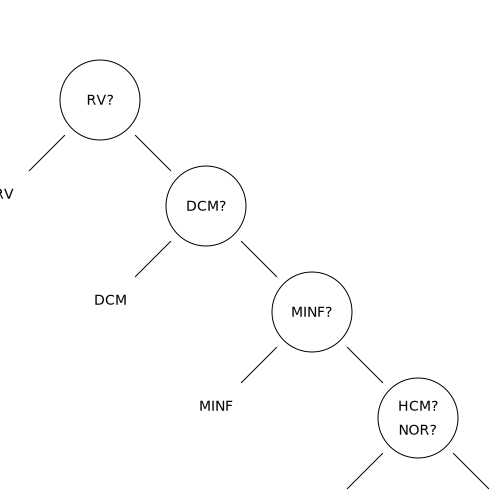
\includegraphics[width=0.5\textwidth]{img/inferencia_cascada}
\caption{Inferencia cascada.}
\end{figure}

\item \textbf{Reuso de \textit{bottleneck}}: En esta idea aunque se reentrenan varios modelos distintos el modelo de partida es el mismo para todos por lo tanto los \textit{bottleneck} se calculan una vez y se usan en todos los pasos como entrada de los modelos que se reentrenan.

%\begin{figure}[H]
%\centering
%\includegraphics[width=0.3\textwidth]{example-image}
%\caption{Reuso de \textit{bottleneck}.}
%\end{figure}

\end{itemize}

Utilizando la técnica descrita anteriormente el resultado es el siguiente:

\begin{table}[H]
\centering
\begin{tabular}{|l|l|l|l|l|l|}
\hline
\textbf{Prueba} & \textbf{Modelo}                   & \textbf{Clases}        & \textbf{Iteraciones}      & \textbf{Learning rate}    & \textbf{Precisión}        \\ \hline
Cascada         & \multicolumn{1}{c|}{inception v3} & \multicolumn{1}{c|}{5} & \multicolumn{1}{c|}{4000} & \multicolumn{1}{c|}{0.01} & \multicolumn{1}{c|}{62.9} \\ \hline
\end{tabular}
\caption{Resultado cascada. Nota: parámetros usados en cada uno de los modelos.}
\end{table}

El resultado de esta prueba es un 62.9\% de precisión que es muy parecido a el mejor resultado que había obtenido hasta ahora (63.2\% de precisión con la prueba, añadir una capa totalmente conectada). Esta prueba no ha supuesto ningún avance ya que se han obtenido resultados muy parecidos a los que ya tenía. Incluso el resultado es ligeramente peor, pero no es significativo ya que puede estar dentro de lo que puede variar la precisión de una ejecución a otra.
\bigskip

Para esta prueba se han implementado los \textit{scripts} \texttt{acdc\_cascade\_test.sh} y \\ \texttt{acdc\_cascade\_batch\_inference.py}. En el primero se hace el entrenamiento de los modelos como se describe anteriormente en este apartado y el otro hace la inferencia de las imágenes de un conjunto. El \textit{script} \texttt{acdc\_cascade\_test.sh} hace usao del \textit{script} \texttt{acdc\_subset\_retrain.py} de la prueba anterior para entrenar los modelos de esta prueba. A continuación se muestra una parte el código principal del \textit{script} \texttt{acdc\_cascade\_test.sh}:

\begin{lstlisting}[language=Bash]
(...)
for step in $(seq 0 $steps); do
  for l in $(seq "$label_count"); do
    set1="$(echo $labels | cut -d ' ' -f $l | tr ' ' ',')"
    set2="$(echo $labels | cut -d ' ' -f $l --complement | tr ' ' ',')"
    subset_retrain "$set1:$set2"
    (...)
    if fgt "$percentage" "$best_percentage"; then
      best_percentage="$percentage"
      best_set1="$set1"
      best_set2="$set2"
    fi
  done
  labels="$(echo $best_set2 | tr ',' ' ')"
  ((label_count--))
done
\end{lstlisting}

Donde la función \texttt{subset\_retrain} hace el entrenamiento de un modelo haciendo uso del \textit{script} \texttt{acdc\_subset\_retrain.py}, donde se pueden ver los parámetros usados para el entrenamiento del modelo. En el \textit{script} \texttt{acdc\_cascade\_test.sh} también se hace uso del \textit{script} \texttt{acdc\_cascade\_batch\_inference.py} para hacer la evaluación.
\bigskip

En el \textit{script} \texttt{acdc\_cascade\_batch\_inference.py} se cargan todos los modelos que se han entrenado haciendo uso de la \textit{api} de \textit{TensorFlow} \texttt{saved\_model} y a continuación se hace la inferencia de las imágenes del conjunto. Se llama a la función \texttt{cascade\_inference()} con cada imagen del conjunto. Esta función se ocupa de hacer la inferencia como se ha descrito anteriormente en este apartado.

\begin{lstlisting}[language=Python]
def cascade_inference(graphs, image_path):
  image_data = tf.gfile.GFile(image_path, 'rb').read()
  for graph, sess, image, prediction, jpeg_data_tensor, decoded_image_tensor, labels, is_last_step in zip(graphs['graph'], graphs['sess'], graphs['image'], graphs['prediction'], graphs['jpeg_data_tensor'], graphs['decoded_image_tensor'], graphs['labels'], graphs['is_last_step']):
    with graph.as_default():
      with sess.as_default():
        resized_image = sess.run(decoded_image_tensor,
                                 {jpeg_data_tensor: image_data})
        result = sess.run(prediction,
                          {image: resized_image})
        label = get_lab(result[0], labels)
        if is_last_step or label == labels[0]:
          return label
\end{lstlisting}

\subsubsection{Inferencia por paciente}
En esta prueba en vez de dar una predicción por \textit{slice} o imagen de un paciente se hace la inferencia en todos las imágenes de un paciente y a continuación se ponen en común todos los resultados y se da como resultado final la clase más repetida en todas las imágenes de cada paciente. También de esta forma se tiene en cuenta que las imágenes están relacionadas por paciente y se da un resultado por cada paciente, no como en pruebas anteriores donde las imágenes que pertenecen a un mismo paciente, podían ser clasificadas como enfermedades distintas.

\begin{table}[H]
\centering
\begin{tabular}{|l|c|c|}
\hline
\textbf{Prueba} & \multicolumn{1}{l|}{\textbf{Sin inferencia por paciente}} & \multicolumn{1}{l|}{\textbf{Con inferencia por paciente}} \\ \hline
Añadir una capa & 63.2                                                      & 71.4                                                      \\ \hline
Cascada         & 62.9                                                      & 57.1                                                      \\ \hline
\end{tabular}
\caption{Resultados inferencia por paciente.}
\end{table}

En este caso se puede ver que en una prueba ha tenido un efecto positivo y en otra ha tenido un efecto negativo. En la prueba, añadir una capa totalmente conectada, hacer la inferencia por paciente ha resultado en una mejora del 8.2\% respecto de la prueba sin hacer la inferencia por paciente lo que es una mejora significativa, mejorando el mejor resultado hasta ahora. Por el contrario en la prueba usando la técnica de cascada ha tenido un efecto negativo.
\bigskip

Para esta prueba se ha implementado el \textit{script} \texttt{per\_patient\_prediction.py} y se han modificado los \textit{scripts} \texttt{batch\_inference.py} y \texttt{acdc\_cascade\_batch\_inference.py}. A los \textit{scripts} modificados se les ha añadido una opción para que guarden en un fichero con formato \texttt{csv} la predicción del modelo y la clase correcta para cada imagen a la que se ha realizado la inferencia.
\bigskip

Después de realizar la inferencia en el conjunto de datos, el \textit{script} \texttt{per\_patient\_prediction.py} lee el fichero \texttt{csv} generado y cuenta para cada paciente la clase más repetida. El \textit{script} muestra por la salida el resultado obtenido y una matriz de confusión.

\subsubsection{Distorsión}
Con el fin de mejorar los resultados hago las mismas pruebas anteriores pero antes aplicando unas transformaciones en todas las imágenes de entrada del \textit{dataset}. En el \textit{dataset} las imágenes de entrada de los pacientes vienen en diferentes posiciones. En este caso las transformaciones que se han realizado a las imágenes es rotarlas 90, 180 y 270 grados cada una.
\bigskip

La distorsión se puede usar en dos casos, en el caso de que los datos del \textit{dataset} de entrada sea reducido y se pretenda aumentar o como en este caso se pretenda que el \textit{dataset} de entrada tenga cierta característica como en este caso en el que las imágenes del \textit{dataset} están rotadas cada una con unos grados. De esta forma se pretende neutralizar que los pacientes en el \textit{dataset} de entrada estén cada uno con una rotación distinta y que los modelos generalicen para aprender a clasificar independientemente de la posición en la que esté la imagen de entrada.

\begin{table}[H]
\centering
\begin{tabular}{|l|c|c|}
\hline
\textbf{Prueba}                             & \multicolumn{1}{l|}{\textbf{Sin distorsión}} & \multicolumn{1}{l|}{\textbf{Con distorsión}} \\ \hline
Añadir una capa                             & 63.2                                         & 57                                           \\ \hline
Añadir una capa con inferencia por paciente & 71.4                                         & 85.7                                         \\ \hline
Usar un slice por paciente                  & 42.9                                         & 35.7                                         \\ \hline
Entrenamiento por subsets (DCM)             & 83.9                                         & 76.2                                         \\ \hline
Entrenamiento por subsets (HCM)             & 76.5                                         & 68.5                                         \\ \hline
Entrenamiento por subsets (MINF)            & 81.6                                         & 84.7                                         \\ \hline
Entrenamiento por subsets (NOR)             & 89.8                                         & 88.9                                         \\ \hline
Entrenamiento por subsets (RV)              & 85.8                                         & 85.2                                         \\ \hline
Cascada                                     & 62.9                                         & 56.3                                         \\ \hline
Cascada con inferencia por paciente         & 57.1                                         & 85.7                                         \\ \hline
\end{tabular}
\caption{Resultados pruebas con distorsión.}
\end{table}

En general la mejora es pequeña en todas las pruebas, excepto en las que la inferencia se hace por paciente. En esas pruebas se obtiene una precisión del 85.7\%.
\bigskip

Para llevar a cabo esta prueba se ha implementado el \textit{script} \texttt{acdc\_distortion.sh}. Este \textit{script} aplica rotación de 90, 180 y 270 grados a cada imagen del \textit{dataset}. La imagen se rota y se guarda en el mismo directorio, de esta forma cuando el \textit{script} del entrenamiento vaya a hacer los conjuntos hará uso de esas imágenes.

\subsubsection{Resultado final}
Después de realizar todas las pruebas descritas en las secciones anteriores los mejores resultados se obtienen en las pruebas realizadas con inferencia por paciente, en concreto con: añadir una capa totalmente conectada y usando la técnica de cascada. Y aplicado distorsión al \textit{dataset} de entrada, en concreto aplicado las transformaciones de rotación de 90, 180 y 270 grados. En ambos casos usando el modelo de partida \textit{inception v3}.

\newpage
\section{Conclusiones y vías futuras}
\subsection{Conclusiones}
En el \textit{machine learning} hay muchos factores que pueden afectar al resultado final, algunos de estos factores son: La arquitectura de la red neuronal. Datos de entrada. Parámetros empleados. Enfoques para resolver un problema, etc. En este trabajo se ha comprobado que todos los factores son importantes a la hora de resolver un problema usando técnicas de \textit{machine learning} y obtener un buen resultado. Por consiguiente, una mala elección de los factores, como una mala repartición del \textit{dataset}, puede llevar a resultados erróneos.
\bigskip

Con la primera prueba realizada en el \textit{dataset} \textit{ACDC} en la que se obtiene un resultado erróneo debido al \textit{overfitting}, usando solo un \textit{slice} por paciente y teniendo en cuenta que el mejor resultado de este trabajo se obtiene aplicando distorsión al \textit{dataset} se cumple el objetivo 1.
\bigskip

%TODO anexo
Se han probado distintos enfoques y configuraciones para resolver el problema como: hacer un entrenamiento completo, añadir solo una capa, añadir 3 capas, quitar capas, usar la técnica de cascada o hacer la inferencia por paciente. Cumpliendo el objetivo 2. Ver Anexo I: Código.
\bigskip

%TODO anexo
Una serie de \textit{scripts} en \textit{python} y \textit{bash} han sido implementados para poder realizar todas pruebas y poder analizar la información. Ver anexo tal. Con esto se cumple el objetivo 3.
\bigskip

Para cumplir el objetivo 4, en el apartado ``Diseño y resolución del trabajo realizado’’ se han juntado los resultados en tablas y se han analizado y comparado los resultados con los de otras pruebas. En cada uno de los apartados correspondiente a cada prueba hay una análisis de esa prueba.
\bigskip

Después de enfocar el problema de diferentes formas, unas con más éxito que otras, se ha conseguido una precisión máxima del 85.7\%, en dos de las pruebas. En concreto en la prueba usando \textit{inception v3} como modelo de partida, añadiéndole una capa totalmente conectada que se reentrena, usando distorsión y haciendo la inferencia por paciente. Y en la prueba usando la técnica de cascada usando como modelo base \textit{inception v3}, usando distorsión y haciendo la inferencia por paciente. De estas dos pruebas se elige como mejor la que usa distorsión y añade solo una capa más al modelo, ya que ha demostrado tener mejor rendimiento también sin usar distorsión y al ser una técnica más simple requiere de menos recursos.

\subsection{Vías futuras}
Algunas de las posibles vías futuras para poder mejorar la precisión son las siguientes:

\begin{itemize}
\item Usar un modelo de partida que procese los datos de entrada en tres dimensiones. Los datos de entrada están formadas por imágenes en tres dimensiones. En este trabajo se han separado las imágenes en una dimensión como imágenes independientes. Usando un modelo con entrada en tres dimensiones, se podrían procesar las imágenes relacionadas juntas por lo que la entrada sería más significativa y aportaría más información en cada muestra del \textit{dataset}.

\item Probar enfocando el problema dividiéndolo en dos pasos primero realizar la segmentación de las partes del corazón y luego usar esa información en conjunto con los datos de entrada para realizar una predicción de la enfermedad.
\end{itemize}


\newpage
\appendix
\addappheadtotoc
\appendixpage
\section{Anexo I: Código}\label{anexo1}
El código de este trabajo se puede encontrar en: \url{https://drive.google.com/drive/folders/1q71pmSSp85m0L4aWFQi78J12YuodHoXS?usp=sharing}.
\bigskip

En el código consiste en una serie de \textit{scripts} que se usan para hacer las pruebas, también hay algunos \textit{scripts} para resumir la información, visualizar los datos y para ejecutarlo todo.
\bigskip

Los \textit{scripts} de \textit{transfer learning} estan basados en el \textit{script} \texttt{retrain.py}.

\begin{itemize}

\item \textbf{Prueba añadir una capa totalmente conectada y \textit{softmax}}

\begin{itemize}
\item \texttt{retrain.py}: aplica la técnica de \textit{transfer learning}.
\end{itemize}


\item \textbf{Prueba añadir 3 capas totalmente conectadas}

\begin{itemize}
\item \texttt{retrain\_3fc.py}: \textit{script} basado en \texttt{retrain.py}, en vez de añadir una sola capa añade 3.
\end{itemize}


\item \textbf{Prueba quitar capas}

\begin{itemize}
\item \texttt{retrain\_3fc.py}: \textit{script} basado en \texttt{retrain.py}, acepta una opción para especificar la capa desde la que se quiere entrenar.
\end{itemize}


\item \textbf{Prueba añadir una capa, sets bien repartidos}

\begin{itemize}
\item \texttt{acdc\_test.sh}: llama a los \textit{scripts} \texttt{retrain.py}, \texttt{batch\_inference.py} y \\ \texttt{per\_patient\_prediction.py}.

\item \texttt{retrain.py}: aplica la técnica de \textit{transfer learning} en el \textit{dataset} \textit{ACDC}.

\item \texttt{batch\_inference.py}: ejecuta la inferencia en todas las imágenes de un conjunto.
\end{itemize}


\item \textbf{Prueba usar un \textit{slice} por paciente}

\begin{itemize}
\item \texttt{acdc\_one\_slice\_test.sh}: llama a los \textit{scripts} \texttt{acdc\_one\_slice\_retrain.py} y \texttt{acdc\_one\_slice\_batch\_inference.py}.

\item \texttt{acdc\_one\_slice\_retrain.py}: aplica la técnica de \textit{transfer learning} en el \textit{dataset} \textit{ACDC} usando solo un \textit{slice} por paciente.

\item \texttt{acdc\_one\_slice\_batch\_inference.py}: ejecuta la inferencia en todas las imágenes de un conjunto.
\end{itemize}


\item \textbf{Prueba entrenamiento por subsets}

\begin{itemize}
\item \texttt{acdc\_subset\_test.sh}: llama a los \textit{scripts} \texttt{acdc\_subset\_retrain.py} y \\ \texttt{acdc\_subset\_batch\_inference.py} una vez por cada clase del \textit{dataset} \textit{ACDC}.

\item \texttt{acdc\_subset\_retrain.py}: aplica la técnica de \textit{transfer learning} en el \textit{dataset} \textit{ACDC}, acepta un parámetro para dividir las clases del \textit{dataset} \textit{ACDC} en subconjuntos.

\item \texttt{acdc\_subset\_batch\_inference.py}: ejecuta la inferencia en todas las imágenes de un conjunto.
\end{itemize}


\item \textbf{Prueba cascada}

\begin{itemize}
\item \texttt{acdc\_cascade\_test.sh}: aplica la técnica de cascada haciendo uso del \textit{script} \\ \texttt{acdc\_subset\_retrain.py} y llama al \textit{script} \texttt{acdc\_cascade\_batch\_inference.py}.

\item \texttt{acdc\_cascade\_batch\_inference.py}: ejecuta la inferencia en todas las imágenes de un conjunto, usando la técnica de cascada.
\end{itemize}


\item \textbf{Prueba inferencia por paciente}

\begin{itemize}
\item \texttt{per\_patient\_prediction.py}: usa los \texttt{csv} generados por los \textit{scripts} de inferencia para dar un resultado por paciente.
\end{itemize}


\item \textbf{Prueba distorsión}

\begin{itemize}
\item \texttt{acdc\_distortion.sh}: aplica rotacion de 90, 180 y 270 grados a todas las imágenes del \textit{dataset} \textit{ACDC}.
\end{itemize}


\item \textbf{Otras pruebas}

\begin{itemize}
\item \texttt{flowers\_test.sh}: llama a los \textit{scripts} \texttt{retrain.py} y \texttt{batch\_inference.py}, con el \textit{dataset} \textit{flowers}.
\end{itemize}


\item \textbf{Otros \textit{scripts}}

\begin{itemize}
\item \texttt{run.sh}: \textit{script} principal que ejecuta todo, prepara los \textit{datasets}, llama a los \textit{scripts} para reunir la información y llama al \textit{script} \texttt{test\_all.sh,} que ejecuta todas las pruebas.

\item \texttt{acdc\_extract.sh}: descomprime el \texttt{zip} del \textit{dataset} \textit{ACDC} y llama al \textit{script} \\ \texttt{acdc\_nii\_to\_jpg.py}.

\item \texttt{acdc\_nii\_to\_jpg.py}: convierte las imágenes del \textit{dataset} \textit{ACDC} que están en formato \texttt{nii} a formato \texttt{jpg}.

\item \texttt{cines.sh}: a partir de las imagenes extraidas del \textit{dataset} \textit{ACDC}, las convierte en videos para poder visualizar el \textit{dataset}.

\item \texttt{info.sh}: genera un \texttt{csv} con la información que se proporciona de cada paciente del \textit{dataset} \textit{ACDC}.

\item \texttt{test\_all.sh}: ejecuta todas las pruebas, el \textit{script} de distorsión, vuelve a ejecutar todas las pruebas y llama al \textit{script} \texttt{summary.sh}.

\item \texttt{summary.sh}: genera un \texttt{csv} donde reúne los resultados de las pruebas ejecutadas.
\end{itemize}

\end{itemize}


\newpage
\nocite{*}
\renewcommand\refname{Bibliografía}
\bibliographystyle{ieeetr}
\bibliography{memoria}

%\clearpage

%\printglossary[type=\acronymtype]

%\newpage
\printglossary[type=\acronymtype,style=long,title={Índice de acrónimos}]

%\printglossaries

\end{document}
